\documentclass[12pt, a4paper,twoside]{tesi_upf}

\usepackage{pgfgantt}
\usepackage{tikz}
\usepackage{eurosym}
\usepackage{float}
\usepackage{pdfpages}

\usetikzlibrary{shapes.geometric, arrows}

\tikzstyle{startstop} = [rectangle, rounded corners, minimum width=3cm, minimum height=1cm,text centered, draw=black, fill=red!30]

\tikzstyle{io} = [trapezium, trapezium left angle=70, trapezium right angle=110, minimum width=3cm, minimum height=1cm, text centered, draw=black, fill=blue!30]

\tikzstyle{process} = [rectangle, minimum width=3cm, minimum height=1cm, text centered, text width=3cm, draw=black, fill=orange!30]

\tikzstyle{decision} = [diamond, minimum width=3cm, minimum height=1cm, text centered, draw=black, fill=green!30]

\tikzstyle{arrow} = [thick,->,>=stealth]

%CODIFICACI�
\usepackage[latin1]{inputenc}


%IDIOMES
\usepackage[catalan,english]{babel}

%NOM�S PER A OBTENIR INDICACI� DEL MARC EN MIDA A4
%\usepackage[cam,a4,center,frame]{crop}

%PER A INCLOURE GR�FICS I EL LOGO DE LA UPF
%\usepackage{graphicx}

\usepackage{caption}
\usepackage{subcaption}

\usepackage{graphicx}

\usepackage{caption}
\usepackage{acronym}
\usepackage{multirow}
%FONTS TIMES O GARAMOND, 
\usepackage{times}
%\usepackage{garamond}
\usepackage{url}

\usepackage{pdfpages}
%SENSE HEADINGS: NO MODIFICAR
\pagestyle{plain}

%PER A L'�NDEX DE MAT�RIES
\usepackage{makeidx}
\makeindex

%ESTIL DE BIBLIOGRAFIA
\bibliographystyle{apalike}


%AQUEST DOCUMENT �S EN CATAL�
\selectlanguage{english}

%EN COMPTES DE �NDEX, LA TAULA DE CONTINGUTS ES TITULA SUMARI
\addto\captionscatalan
  {\renewcommand{\contentsname}{\Large \sffamily Sumari}}

% ~~~~~~~~~~~~~~~~~~~~~~~~~~
% CUSTOM PACKAGES
% ~~~~~~~~~~~~~~~~~~~~~~~~~~
%\usepackage{hyperref}
\usepackage[hidelinks]{hyperref}
\usepackage{titlesec}
\setcounter{secnumdepth}{4}
\usepackage{pdfpages}

%AFEGIU EN AQUESTA PART LES VOSTRES DADES
\title{A bottom up sensor testbed}
\author{Sergio Almendros D�az}
\thyear{2014}
\department{Departament de Tecnologies de la Informaci� i les Comunicacions (DTIC)}
\supervisor{Jaume Barcel�}


\begin{document}

\pdfstringdefDisableCommands{%
\let\MakeUppercase\relax
}

\frontmatter

\maketitle

\cleardoublepage


%%%%%% Dedicat�ria; si no es vol posar, comenteu fins a final de dedicat�ria

%\noindent Dedicat�ria

%\cleardoublepage

%%%%%% Final de dedicat�ria


%%%%%% Agra�ments; si no es vol posar, comenteu fins a final de agra�ments
\noindent {\Large \sffamily Acknowledgments}


\cleardoublepage

%%%%%% Final dels agra�ments

%ABSTRACT EN DOS IDIOMES. COM A M�NIM CATAL�. SI L'ALTRE �S EN CASTELLA CANVIEU EL QUE POSA ABSTRACT
\selectlanguage{english}
\section*{\Large \sffamily Abstract}

  This project aims to deploy a sensor node network prototype taking advantage of the guifi network, an open, free and neutral network, and the visualization of this data in an intuitive and meaningful way, tailoring the presentation of the data to people without specific scientific knowledge.
  
  The main objective is to give citizens a trace to improve environmental conscience, giving them the necessary information to know the state of their environment and so they can act accordingly.
  This way anybody can act consequently if the sensors detect harmful situations, for example, not going to a park where the gas sensor detects bad air quality.
   
  From this point, Arduino Yun is the main component of the sensor node. Through a series of sensors attached to it and the Internet connection provided by guifi, the node can communicate with a storage platform for sensor data, in this case, Opencities. Finally, an Android application downloads the sensor data from Opencities and display them on a map.


\selectlanguage{catalan}
\vspace*{\fill}
\section*{\Large \sffamily  Resum}

Cuando el Abstract est� perfecto, lo traducir� al catalan.

\vspace*{\fill}

\selectlanguage{english}
\cleardoublepage
%FIN DE ABSTRACTE

%PREFACI OPCIONAL. SI NO ES VOL, COMENTEU FINS EL FINAL DE PREFACI
%{\bf Prefaci}
%
%\cleardoublepage
%FINAL DE PREFACI


%TAULA DE CONTINGUTS: OBLIGAT�RIA
\selectlanguage{english}
\tableofcontents

%INDEX DE FIGURES; NOM�S ES POSA SI HI HA FIGURES
\listoffigures
%Fa que aparegui al sumari
\addcontentsline{toc}{chapter}{List of figures}

%INDEX DE TAULES; NOM�S ES POSA SI HI HA TAULES
%\listoftables
%Fa que aparegui al sumari
%\addcontentsline{toc}{chapter}{List of tables}


%COMEN�A EL TEXT
\mainmatter
\chapter{Introduction}
\label{Chapter1}

  The development of this project has been divided into three phases: collect data from environmental sensors, display it to end users in an intuitive way, and make a real testbed to demonstrate its performance.
  
  As a sensor node has been used an Arduino\cite{arduino} YUN, which allows to obtain easily analog reads from a sensor and, with a Power over Ethernet module, it can be attached to Guifi\footnote{\url{http://guifi.net/}} nodes and send the sensor data to a sensor platform, e.g. Opencities \cite{opencities}.

  The Bottom-up\footnote{\url{http://bubforeurope.net}} pattern has been used to build the sensor testbed, where the end users, in this case, guifi users, are the ones who have to assemble the sensor nodes and connect them to their guifi nodes to create the sensor network. With the bottom-up model, the data is provided and used by the end users.

  In this project an Android application has been developed to visualize the sensor data and make it accessible to the end users.
  A sensor testbed has been deployed to gather sensor data, and test the technologies used as nodes.
  
  This project is an attempt to understand the structure, the technological challenges and operations of sensor networks and how they can help us to take conscience about our environment.

  The thesis is structured as follows: the actual state of sensor networks (Chapter \ref{Chapter2}), which technologies had been used (Chapter \ref{Chapter3}), and how the project has been developed (Chapter \ref{Chapter4}). 
  In chapter \ref{Chapter5} the testbed deployment is illustrated and some resulting data are shown.
  Finally, the conclusions (Chapter \ref{Chapter6}) and future work (Chapter \ref{Chapter7}).
  
\chapter{State of the Art}
\label{Chapter2}
  
  \section{Introduction}
    Sensor networks started as a mecanism of defense developed by the United States Navy during the Cold War, with acoustic sensors they searched for Soviet submarines. This search continued at Universities, trying to make the sensors smaller, and with the posibility of real-time data \cite{chong2003sensor}.
    
    Sensor networks should not affect the environment, in our case, visually. For this purpose we must ensure that the nodes are relatively small, so the board and sensors had been selected accordingly.
    
    To choose the processor board, it has to be look into the following characteristics:
    
    \begin{itemize}
    	\item {\bf Power:} A sensor node can obtain energy in several ways: batteries, solar energy, connecting to an alredy deployed network... The important thing is not to increase the size of the sensor, in our case, is power by an already deployed network.
    	\item {\bf CPU:} A powerful CPU is not necessary to process sensor data, so this helps to decrease the size of the board and reduce power consumption.
    	\item {\bf Communication:} There has to be a way to send the collected data outside, usually wireless or through a wired network. If it has wireless communication, the topology and location of the sensor nodes has to be chosen properly. But if it is through a wired network, it should take advantage of something already deployed. In our case, the guifi network is already deployed.
    \end{itemize}
    
    Currently the sensors are small enough to take several together with the same size as the board mentioned before.
    
    Smart cities are the next step. A city capable of having real-time information, not only about the environment, but also from the number of cars that pass on a road, to the amount of rain water in a day. This kind of information could help to manage more efficiently the city.
    
    It is important to share this information so everyone can know the state of their environment. There are already some sensor networks functioning, some of them are government-funded and they often apply a policy where the data is not completel public, while other sensor networks are private-owned and the data are possibly open (e.g. smartcitizen).

  \section{Sensor networks and smart cities}
    In this section a few projects on sensor networks deployed has been introduced:
    
    \subsection{Amsterdam smart city}
      Amsterdam has many projects concerning the smart city concept, like the ``Flexible street lighting'', which allows the government to monitor the street and switch off the lights to save energy, or the ``Smart parking'' which let drivers to know if there are free spots to park, and, in consecuence, reduce air pollution \cite{SmartcityAmsterdam}.
      
    \subsection{Santander smart city}
      Santander has his own sensor network testbed for environmental monitoring, outdoor parking area management, and traffic intensity monitoring \cite{SmartcitySantander}.
    
  \section{Companies}
    In the following sections some companies that are in the business of sensor networks are described.
    
    \subsection{Smartcitizen}
      Smart Citizen\footnote{\url{http://www.smartcitizen.me/}} is platform that offers a sensor board based on Arduino to monitor the environment (figure \ref{fig:SmartCitizenNode}), and permits to upload this data to their own public database.
      
      \begin{figure}[htbp]
        \centering
            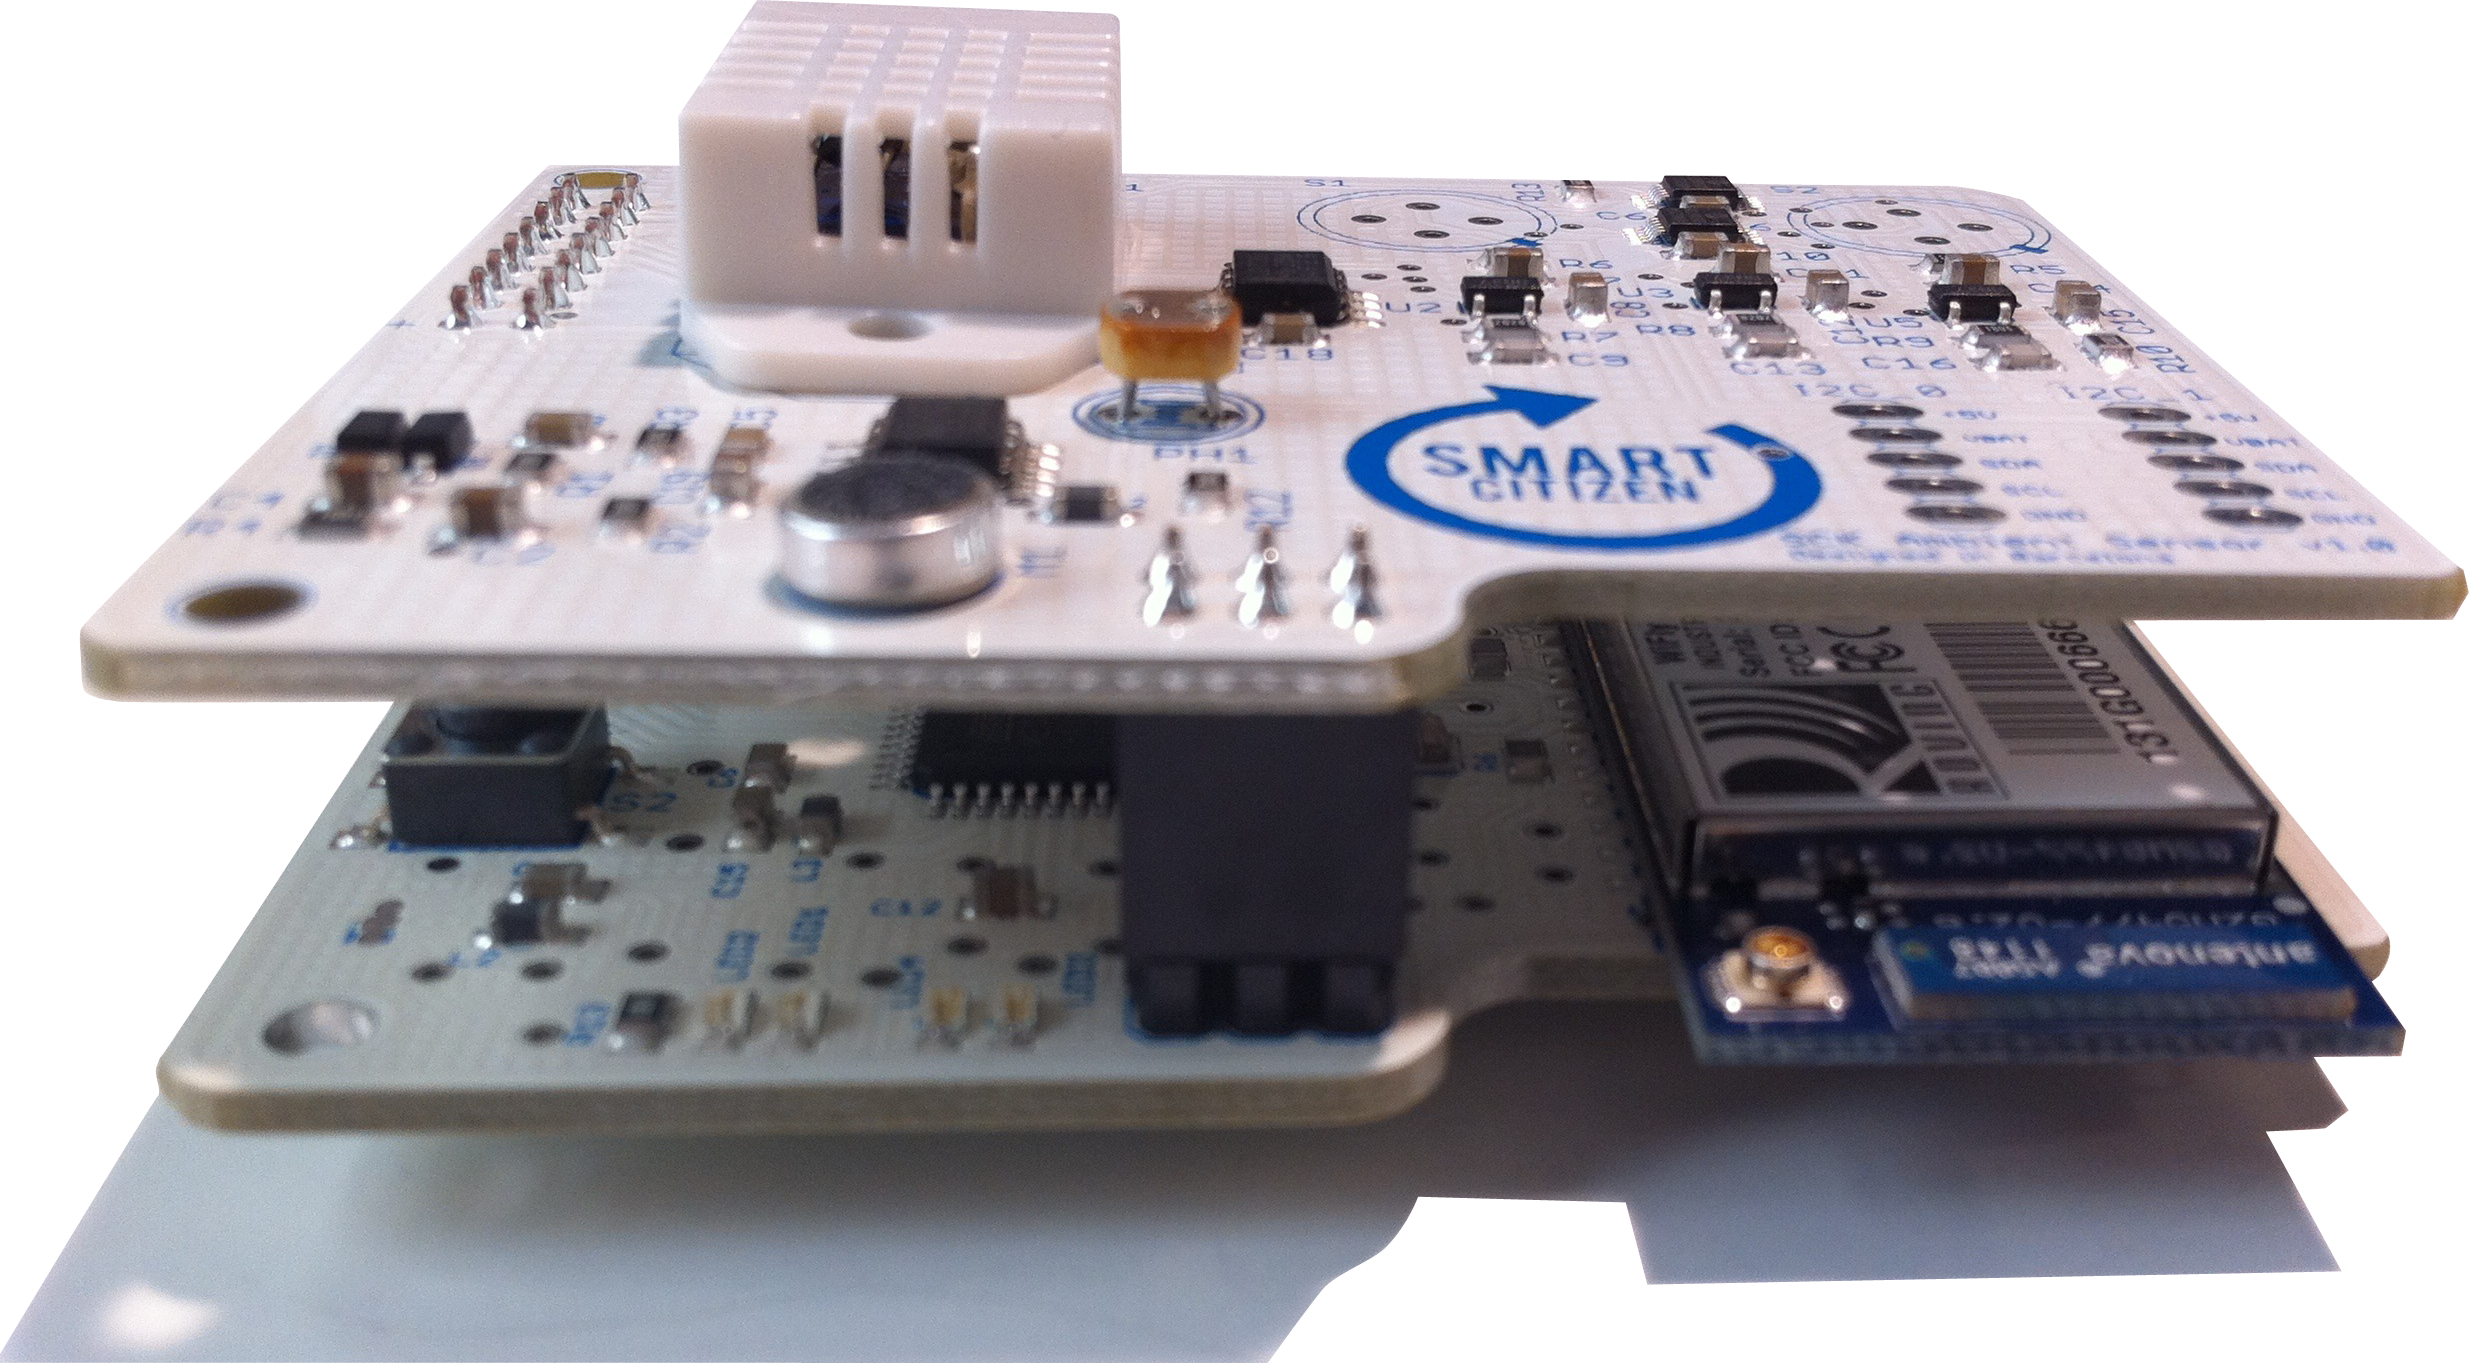
\includegraphics[scale=0.08]{./Figures/smartcitizen.png}
            \rule{18em}{0.5pt}
        \caption[Smart Citizen Node]{Smart Citizen Node.}
        \label{fig:SmartCitizenNode}
    \end{figure}
            
    \subsection{Libelium}
      Libelium is an Internet of things platform provider\footnote{\url{http://www.libelium.com/}}, which supplies an open source sensor platform for the Internet of things.
      They have a variety of products, some interesting ones are shown:
      \begin{itemize}
        \item e-Health: A sensor shield for Arduino and Raspberry Pi for body monitoring: pulse, oxygen in blood, airflow (breathing), body temperature, electrocardiogram, glucometer, galvanic skin response, blood pressure, patient position, and muscle/eletromyography sensor (Figure \ref{fig:Libeliumehealth}).
        
        \item Waspmote: A sensor node where it is possible attach more than 60 sensors, solar powered, and though to fit onto street light poles. (Figure \ref{fig:LibeliumWaspmote}).
       
       \item Smart Water: A wireless sensor platform for water quality monitoring, it provides real-time data. (Figure \ref{fig:LibeliumSmartWater}).
     \end{itemize}
      
      \begin{figure}
        \centering
        \begin{subfigure}[b]{0.3\textwidth}
                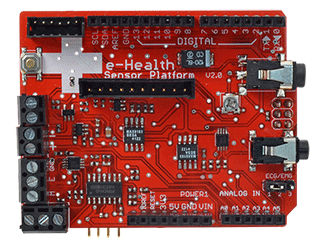
\includegraphics[width=\textwidth]{./Figures/Libeliume_health.png}
                \caption{Libelium ehealth}
                \label{fig:Libeliumehealth}
        \end{subfigure}%
        ~ %add desired spacing between images, e. g. ~, \quad, \qquad, \hfill etc.
          %(or a blank line to force the subfigure onto a new line)
        \begin{subfigure}[b]{0.3\textwidth}
                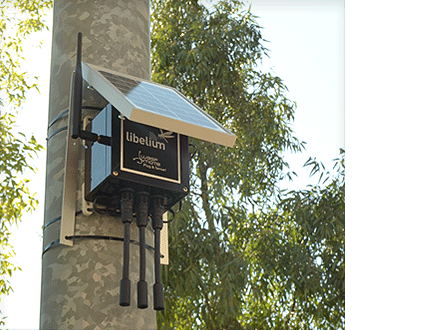
\includegraphics[width=\textwidth]{./Figures/LibeliumWaspmote.png}
                \caption{Libelium Waspmote}
                \label{fig:LibeliumWaspmote}
        \end{subfigure}
        \begin{subfigure}[b]{0.3\textwidth}
                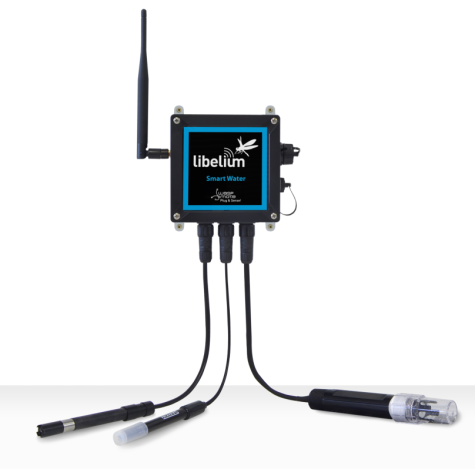
\includegraphics[width=\textwidth]{./Figures/LibeliumSmartWater.png}
                \caption{Libelium Smart Water}
                \label{fig:LibeliumSmartWater}
        \end{subfigure}
        \rule{18em}{0.5pt}
        \caption{Libellium Projects}\label{fig:LibelliumProjects}
		\end{figure}
      
           
    
  \section{Opendata services}
    The sensor boards are continuosly collecting data, which has to be stored. The data can be stored locally or remotly. Collecting the data from the sensor board it is unpractical. For this reason an online storage service, opendata, is needed.    
    
		\subsection{Opencities}
       Opencities \cite{opencities} is a platform to browse, visualize, and download open data from different participants. Opencities has very simple API to upload and download data, a web page to visualize the stored data.
       
       and the possibility that the project can contribute to their system, and so they to the project.
       
    \subsection{Xively}
      Xively \footnote{\url{https://xively.com}} offers an Internet of Things platform as a service, basically it lets you store sensor data, download it, and visualize it through graphics.
    
    \subsection{Sentilo}
      Sentilo \footnote{\url{http://www.sentilo.io}} is a open source platform for Smart Cities, it allows the user to use their own service to store the data, but they do not intend to become the database for everyone, it is only as an example. The Sentilo platform does not depend on a central server and can be installed on a private server. It also provides a interface to show the data.
    
  \section{Sensor boards}
    In this section are discussed some of the options for a sensor node.
    
    \subsection{Arduino YUN}
      The Arduino YUN is a microcontroller board with two processors (figure \ref{fig:AYUN}), an ATmega32u4 (Arduino), and an Atheros AR9331 (Whhich runs a Linux distribution named OpenWrt-Yun). It has an Ethernet and WiFi module, a USB-A port, a micro-SD card slot, 20 digital input/ouput ping, 16 MHz crystal oscillator, ICSP header, and 3 reset buttons.
      \begin{figure}[htbp]
        \centering
            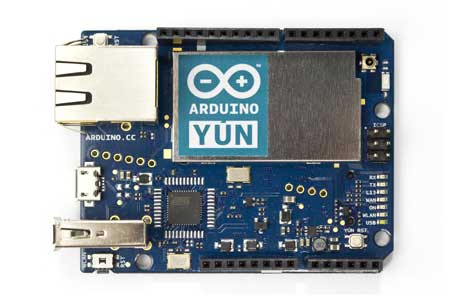
\includegraphics[scale=0.4]{./Figures/ArduinoYunFront_2_450px.jpg}
            \\
            \rule{15em}{0.5pt}
        \caption[Arduino YUN]{Arduino YUN.}
        \label{fig:AYUN}
      \end{figure}
      
      The peculiarity about the Arduino YUN is that the processor for the Arduino sketches can communicate with the Linux processor through the bridge library, which allows you to write python scripts and execute them (figure \ref{fig:BridgeInShort}).
      
      A power over ethernet module (PoE) can be attach to the Arduino, which has a particular interest for the guifi network, where the antennas are powered through PoE.
      \begin{figure}[htbp]
          \centering
              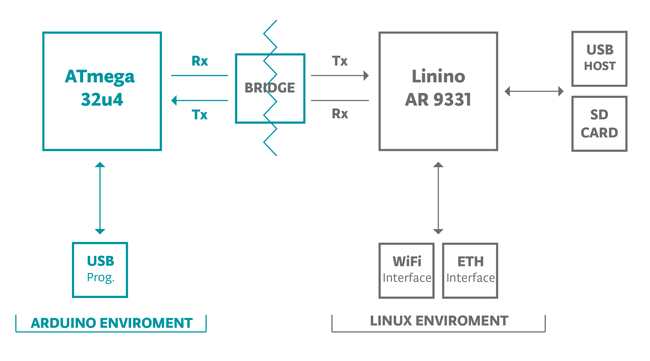
\includegraphics[scale=0.5]{./Figures/BridgeInShort.png}
              \\
              \rule{23em}{0.5pt}
          \caption[Arduino YUN Bridge]{Arduino YUN Bridge.}
          \label{fig:BridgeInShort}
       \end{figure}
        
    \subsection{Raspberry Pi}
      Raspberry Pi\footnote{\url{http://www.raspberrypi.org/}} is a single-board computer, produced in two models, A and B. The model B (Figure \ref{fig:RaspberryPiB}) is more appropiate for this project because it has an Ethernet controller. It is composed by an HDMI, a micro USB, an USB 2.0 connector, an SD card slot, Input/Output (GPIO) pins, an RCA connector, an audio jack, an Ethernet controller, and a Broadcom BCM2835 processor.
     
      It is possible to attach sensors to it, and it supports Linux environment.
      \begin{figure}[htbp]
          \centering
              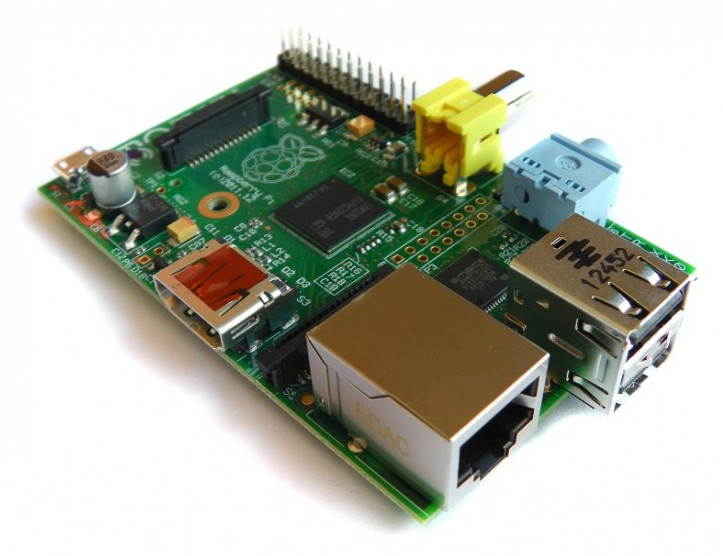
\includegraphics[scale=0.2]{./Figures/raspberry-pi-model-b.jpg}
              \\
              \rule{15em}{0.5pt}
          \caption[Raspberry Pi model B]{Raspberry Pi model B.}
          \label{fig:RaspberryPiB}
       \end{figure}
    
    \subsection{Picoboard}      
      PicoBoard\footnote{\url{http://www.picocricket.com/picoboard.html}} is a board to interact with the world, it can be programmed by Scratch projects. It is less flexible than the previously mentioned, it is composed by a button, a light and a sound sensor, a slider, and alligator clips which can be use to build custom sensors. This board can be seen in the figure \ref{fig:picoboard}.
      
      \begin{figure}[htbp]
          \centering
              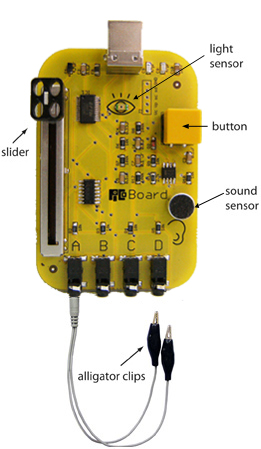
\includegraphics[scale=0.5]{./Figures/picoboard.jpg}
              \\
              \rule{16em}{0.5pt}
          \caption[Picoboard]{Picoboard.}
          \label{fig:picoboard}
       \end{figure}

\chapter{Technologies}
\label{Chapter3}
  
  This chapter is focused on the techonologies used to develop this project.
  
  \section{Arduino-Raspberry PI comparison}
    For this project, two possible boards have been considered: the Arduino Yun (Yun) and the Raspberry Pi model B (RPiB).
    
    The Yun is a microcontroller while the RPiB is a full computer, which makes it more powerful, even more than needed, so both Yun and RPiB serve.
    
    The two of them have a Linux environment, but with the Yun, the normal way to interact is by an Arduino sketch. So RPiB considers that the developer has some prior Linux knowledge, while the Yun is better for beginners. Because the Arduino IDE provides a variety of programs that help to start.
    
    The sensor board is the biggest element of the sensor node, so the size is very important, the smaller the better. In this case, the Yun is smaller than the RPiB. On the other hand, the sensor node will be attach on guifi nodes, which are powered by Power over Ethernet (PoE). 
    For the Yun there is the posibility of a PoE module which it is not available yet, which will power the board. The figure \ref{fig:arduinoethernetpoe} and \ref{fig:poerpi} show the comparison between the size of an Arduino Ethernet (similar to the YUN) and the RPiB both powered by PoE. It is clearly visible that the Arduino is more compact.
    
    \begin{figure}
        \centering
        \begin{subfigure}[b]{0.3\textwidth}
                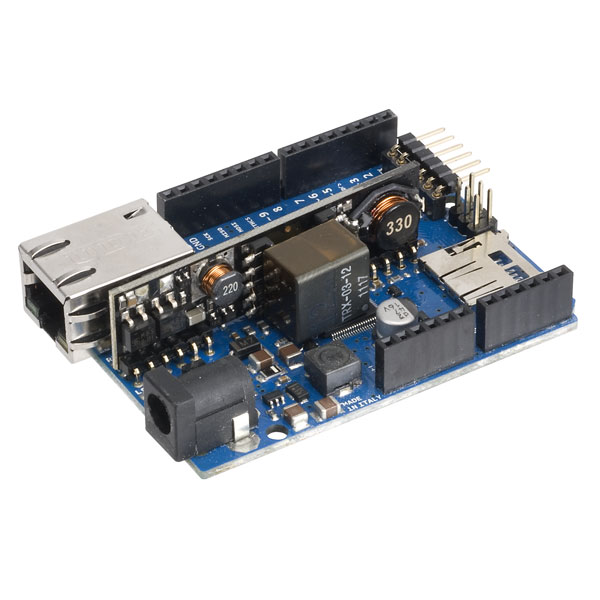
\includegraphics[width=\textwidth]{./Figures/arduinoethernetpoe.jpg}
                \caption{Arduino Ethernet PoE}
                \label{fig:arduinoethernetpoe}
        \end{subfigure}%
        ~ %add desired spacing between images, e. g. ~, \quad, \qquad, \hfill etc.
          %(or a blank line to force the subfigure onto a new line)
        \begin{subfigure}[b]{0.3\textwidth}
                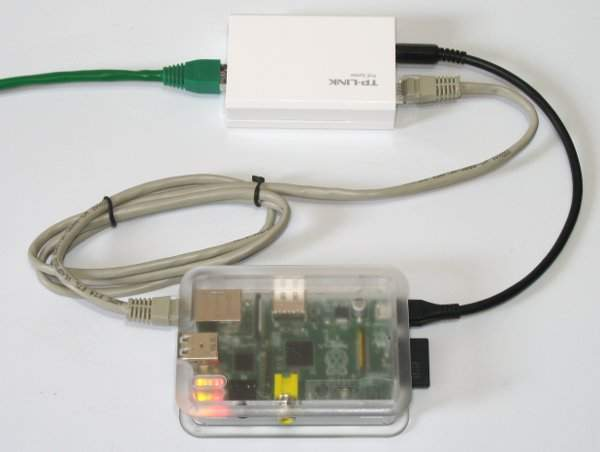
\includegraphics[width=\textwidth]{./Figures/poe-rpi.jpg}
                \caption{Raspberry Pi (B) PoE}
                \label{fig:poerpi}
        \end{subfigure}
        \rule{18em}{0.5pt}
        \caption{Sensor boards}\label{fig:sensorboards}
		\end{figure}

    Another advantage that YUN offers is the integrated WiFi module, which offers more flexibility when there is no ethernet available.
    
    Finally, the Arduino Yun has been used instead of the Raspberry Pi basically because of the size that will become the sensor node, but if in the future will be necessary a more powerful processor, it will be better to use a Raspberry Pi.  

  \section{Sensors}
    The goal is to analyze the environment around us, for that purpose, sensors are a mean to detect physical or chemical variables. It has been decided to use of low cost environmental sensors that are easily accessible and usable. 
    These sensors measure the aspects that may be more useful for citizens: temperature, light, noise, humidity, and air quality.
    
    A sensor is a device which transform a physical measure to an output signal (Voltage or Digits) that can be read by another device, such as an Arduino.
    In this project we will use five sensors that measured temperature, light, noise, humidity, and gas.
    To show how the sensors are connected to the Arduino YUN the program fritzing\footnote{\url{http://fritzing.org/}} has been used.
    
    \subsection{LM35: Temperature}
      LM35 [Figure \ref{fig:LM35}] is a sensor to mesure temperature, in the figure \ref{fig:TemperatureSensor_bb} is shown how to connect it to the Arduino.
      \cite{LM35}
      %\TwoFig{./Figures/LM35.jpg}{LM35 sensor}{fig:LM35}{./Figures/Fritzing/TemperatureSensor_bb.png}{Temperature Sensor Breadboard}{fig:TemperatureSensor_bb}
      
      \begin{figure}
        \centering
        \begin{subfigure}[b]{0.3\textwidth}
                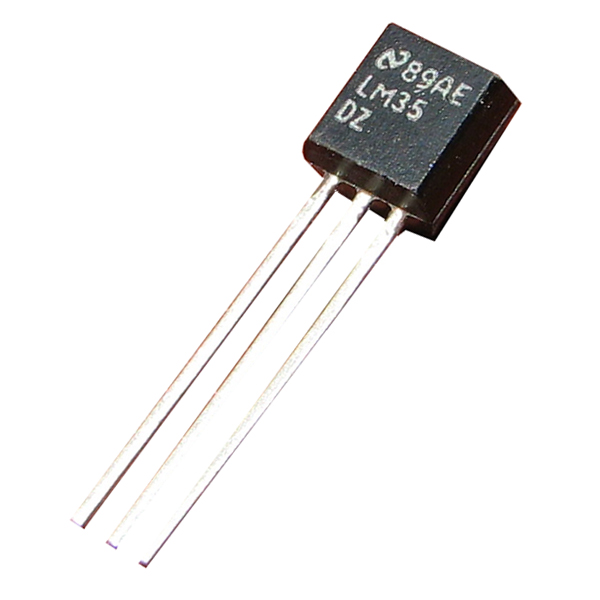
\includegraphics[width=\textwidth]{./Figures/LM35.jpg}
                \caption{LM35 sensor}
                \label{fig:LM35}
        \end{subfigure}%
        ~ %add desired spacing between images, e. g. ~, \quad, \qquad, \hfill etc.
          %(or a blank line to force the subfigure onto a new line)
        \begin{subfigure}[b]{0.3\textwidth}
                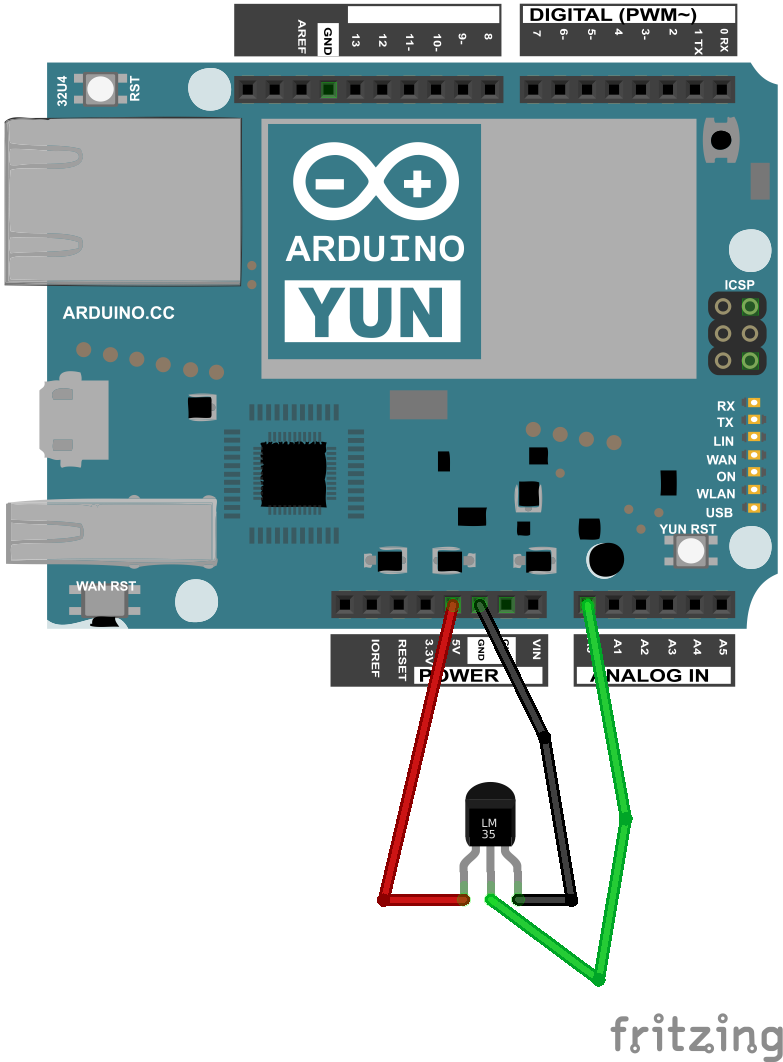
\includegraphics[width=\textwidth]{./Figures/Fritzing/TemperatureSensor_bb.png}
                \caption{Temperature Sensor Breadboard}
                \label{fig:TemperatureSensor_bb}
        \end{subfigure}
        \rule{18em}{0.5pt}
        \caption{Temperature sensor}\label{fig:temperaturesensor}
		\end{figure}
      
    \subsection{Light Dependent Resistor (LDR)}
      LDR [Figure \ref{fig:LDR}] is a light sensor, in the figure \ref{fig:LightSensor_bb} is depicted how to connect it to the Arduino.
      
      \begin{figure}
        \centering
        \begin{subfigure}[b]{0.3\textwidth}
                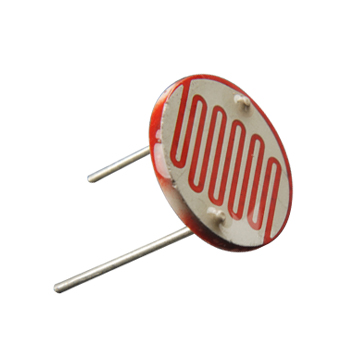
\includegraphics[width=\textwidth]{./Figures/LDR.jpg}
                \caption{LDR sensor}
                \label{fig:LDR}
        \end{subfigure}%
        ~ %add desired spacing between images, e. g. ~, \quad, \qquad, \hfill etc.
          %(or a blank line to force the subfigure onto a new line)
        \begin{subfigure}[b]{0.3\textwidth}
                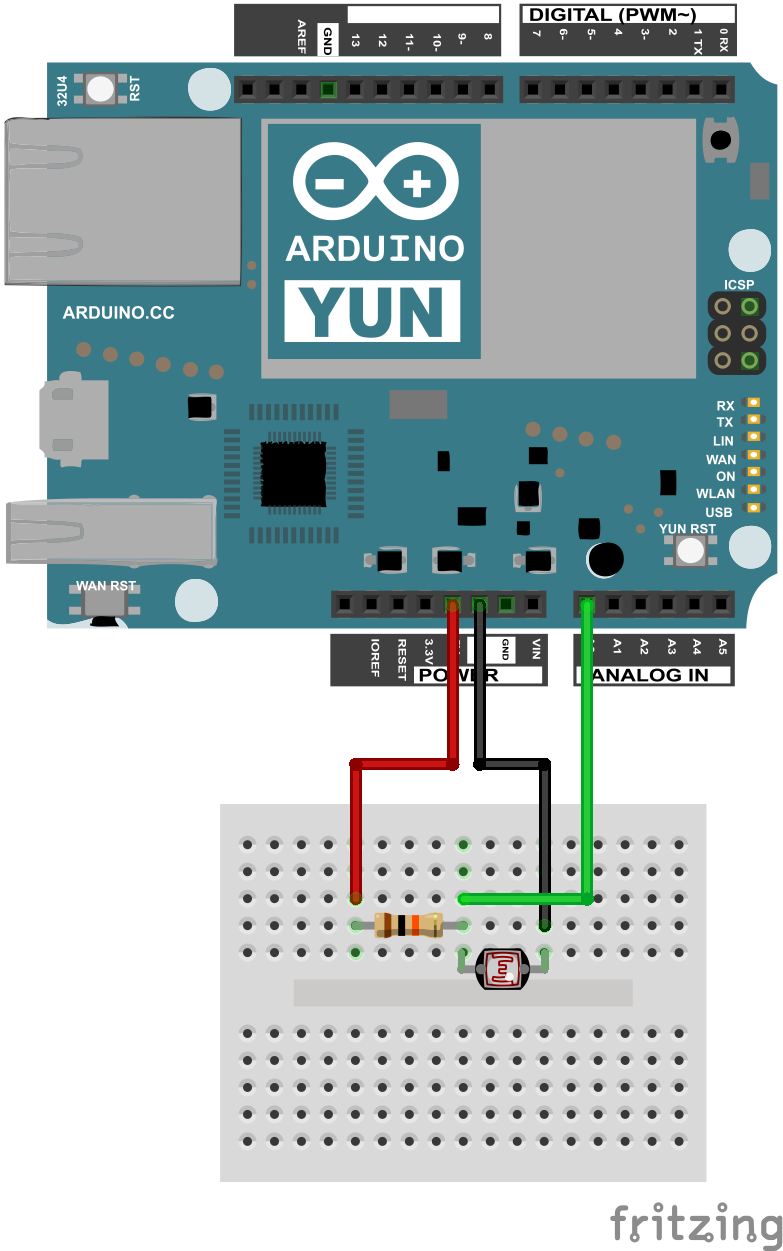
\includegraphics[width=\textwidth]{./Figures/Fritzing/LightSensor_bb.png}
                \caption{Light Sensor Breadboard}
                \label{fig:LightSensor_bb}
        \end{subfigure}
        \rule{18em}{0.5pt}
        \caption{Light sensor}\label{fig:lightsensor}
			\end{figure}
 
    \subsection{Emartee Mini Sound Sensor and Analog Sound Sensor Board Microphone MIC Controller: Noise}
      This two sensors \cite{emarteeminisound} are used to measured noise levels [Figure \ref{fig:MSS}] and [Figure \ref{fig:Analognoisesensor}]. The code to read the noise values is the same for both. In the figure \ref{fig:NoiseSensor_bb} is shown how to connect them to the Arduino.
      
      \begin{figure}
        \centering
        \begin{subfigure}[b]{0.3\textwidth}
                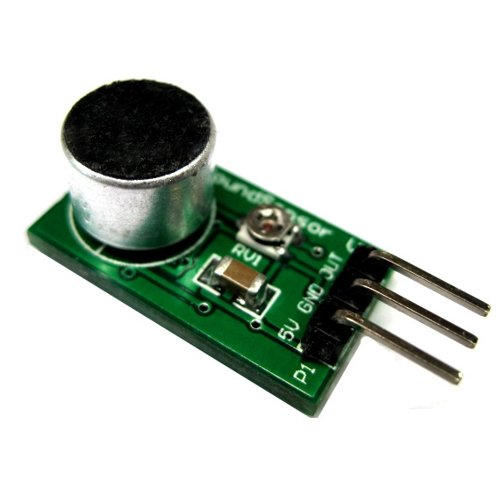
\includegraphics[width=\textwidth]{./Figures/MiniSoundSensor.jpg}
                \caption{Mini Sound Sensor}
                \label{fig:MSS}
        \end{subfigure}%
        ~ %add desired spacing between images, e. g. ~, \quad, \qquad, \hfill etc.
          %(or a blank line to force the subfigure onto a new line)
        \begin{subfigure}[b]{0.3\textwidth}
                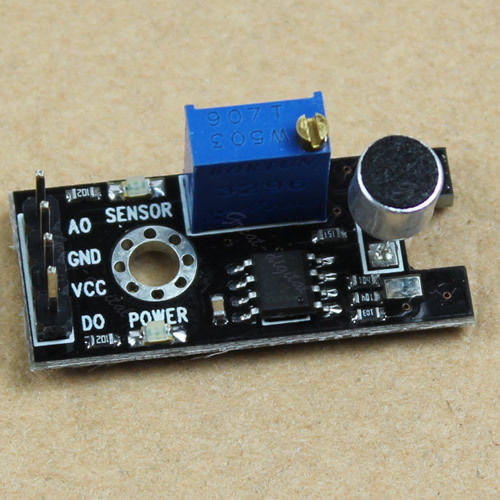
\includegraphics[width=\textwidth]{./Figures/analognoisesensor.jpg}
                \caption{Analog noise sensor}
                \label{fig:Analognoisesensor}
        \end{subfigure}
        \begin{subfigure}[b]{0.3\textwidth}
                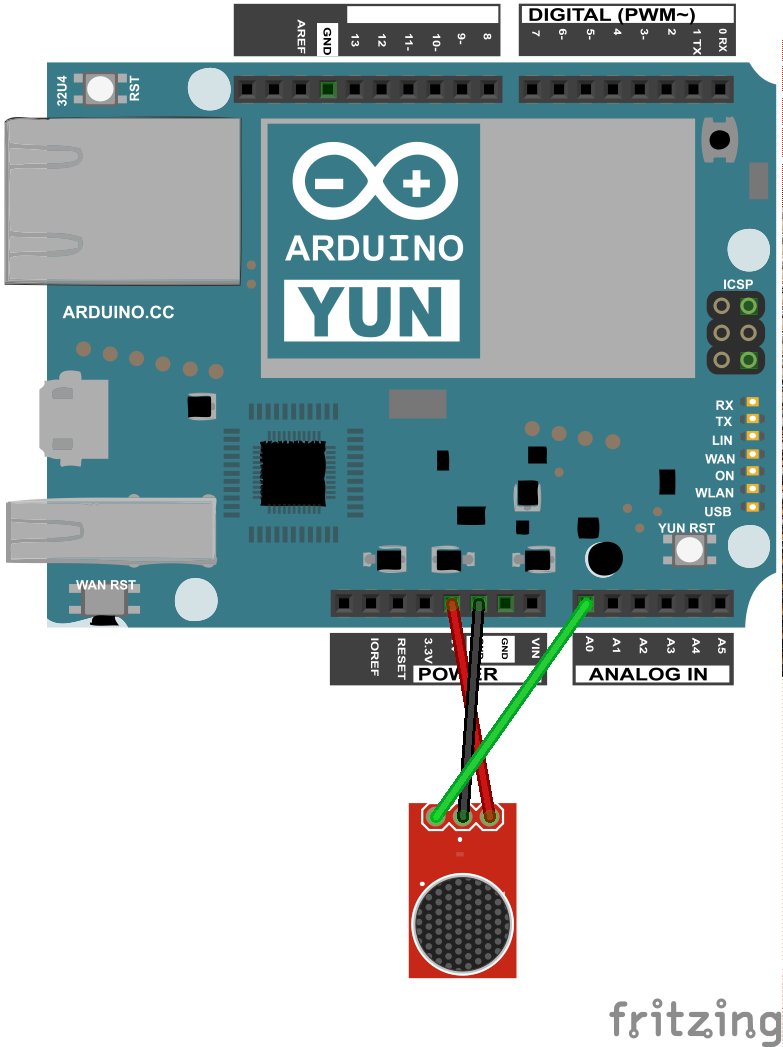
\includegraphics[width=\textwidth]{./Figures/Fritzing/NoiseSensor_bb.png}
                \caption{Noise Sensor Breadboard}
                \label{fig:NoiseSensor_bb}
        \end{subfigure}
        \rule{35em}{0.5pt}
        \caption{Noise sensor}\label{fig:noisesensor}
			\end{figure}


    \subsection{Aosong DHT22 and DHT11: Humidity}
      DHT22 [Figure \ref{fig:DHT22}] and DHT11 [Figure \ref{fig:DHT11}] are humidity and temperature sensors, although the humidity measure is the only one used. The output is digital, and to read it, an external library\footnote{\url{https://github.com/adafruit/DHT-sensor-library}} is needed. The Arduino and the humidity sensor have to be connected as shown in the figure \ref{fig:HumiditySensordht22_bb} for the DHT22 and as shown in the figure \ref{fig:HumiditySensordht11_bb} for the DHT11 \cite{dht22sensor}.
      
      \begin{figure}
        \centering
        \begin{subfigure}[b]{0.3\textwidth}
                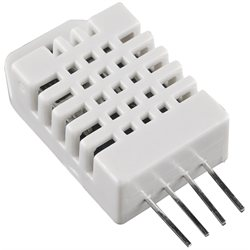
\includegraphics[width=0.8\textwidth]{./Figures/dht22.jpg}
                \caption{DHT22 sensor}
                \label{fig:DHT22}
        \end{subfigure}%
        ~ %add desired spacing between images, e. g. ~, \quad, \qquad, \hfill etc.
          %(or a blank line to force the subfigure onto a new line)
        \begin{subfigure}[b]{0.3\textwidth}
                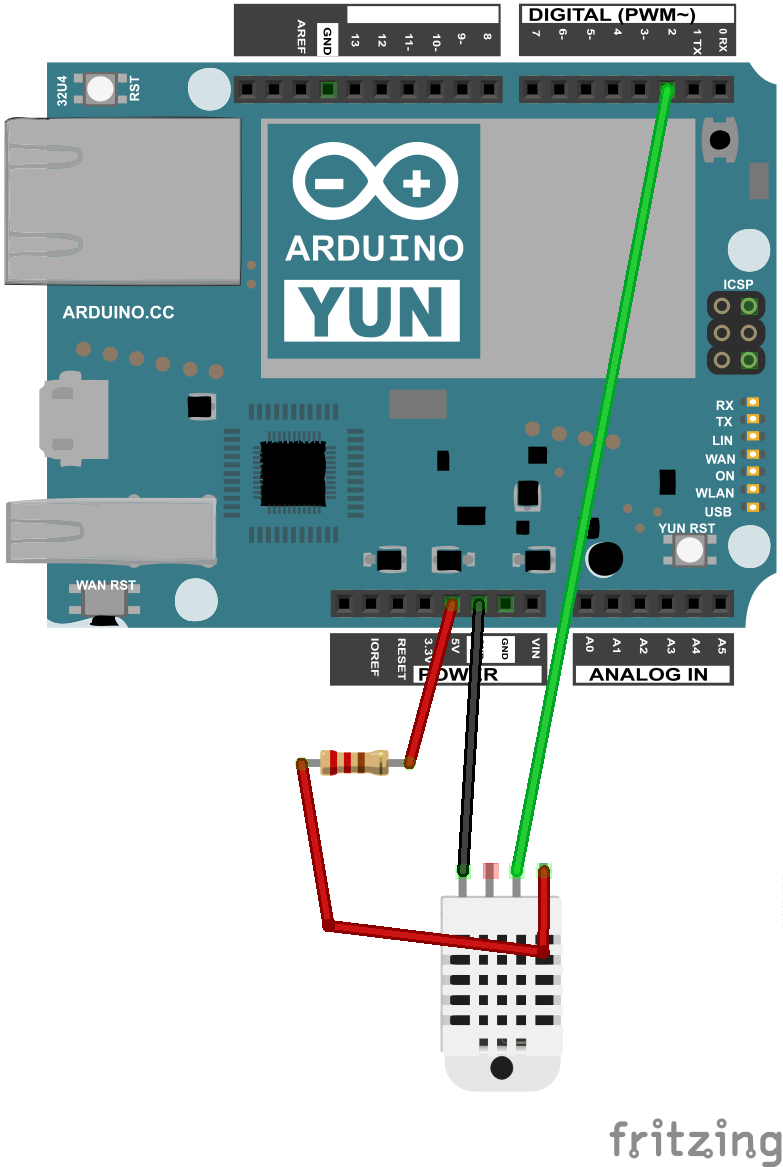
\includegraphics[width=\textwidth]{./Figures/Fritzing/HumiditySensor_bb.png}
                \caption{DHT22 Sensor Breadboard}
                \label{fig:HumiditySensordht22_bb}
        \end{subfigure}
        \rule{18em}{0.5pt}
        \caption{DHT22 sensor}\label{fig:DHT22sensor}
			\end{figure}
      
      \begin{figure}
        \centering
        \begin{subfigure}[b]{0.3\textwidth}
                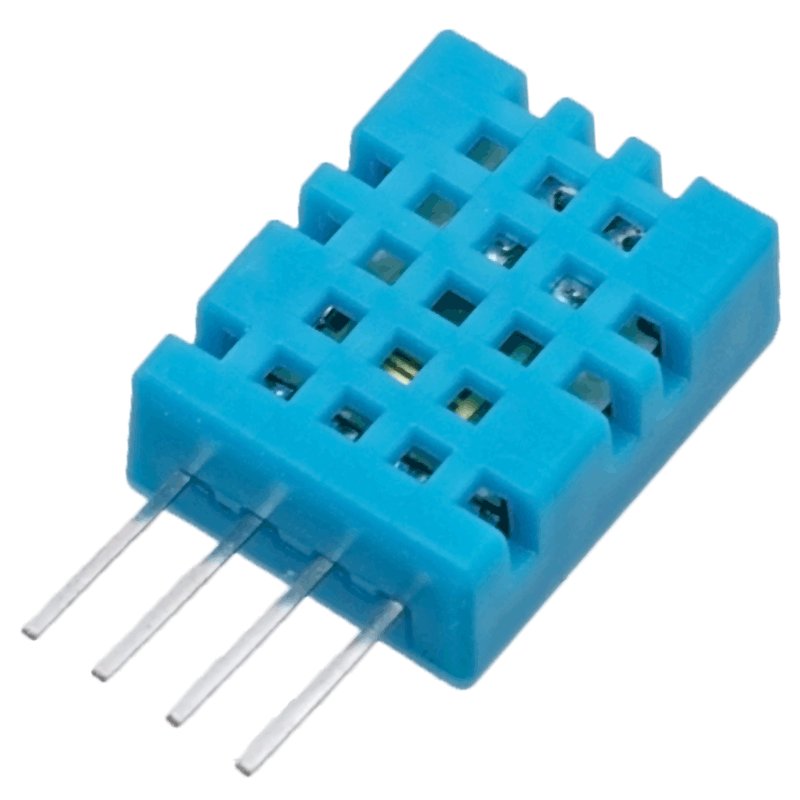
\includegraphics[width=0.7\textwidth]{./Figures/dht11.png}
                \caption{DHT11 sensor}
                \label{fig:DHT11}
        \end{subfigure}%
        ~ %add desired spacing between images, e. g. ~, \quad, \qquad, \hfill etc.
          %(or a blank line to force the subfigure onto a new line)
        \begin{subfigure}[b]{0.3\textwidth}
                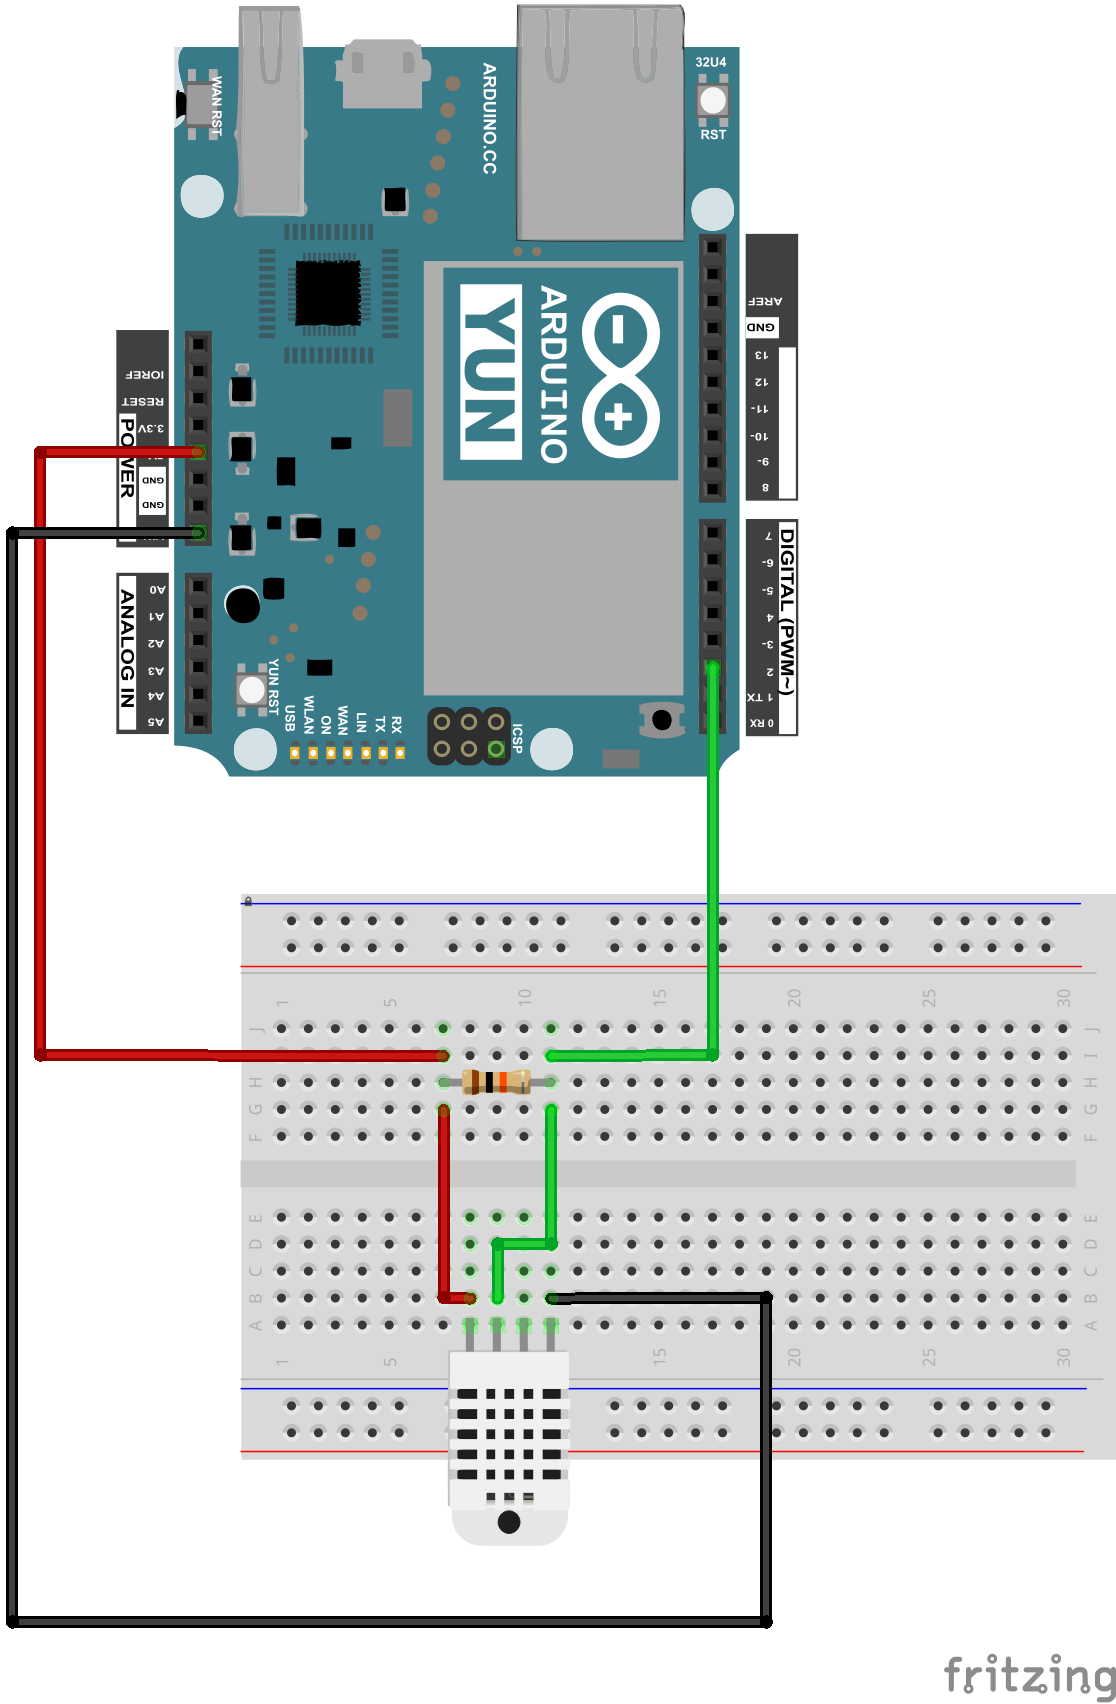
\includegraphics[width=\textwidth]{./Figures/Fritzing/HumiditySensorDht11_bb.png}
                \caption{DHT11 Sensor Breadboard}
                \label{fig:HumiditySensordht11_bb}
        \end{subfigure}
        \rule{18em}{0.5pt}
        \caption{DHT11 sensor}\label{fig:DHT11sensor}
			\end{figure}     
      
    \subsection{MQ135: Gas sensor}
      MQ135 is a gas sensor [Figure \ref{fig:MQ135}], and is used to measure air quality. Figure \ref{fig:GasSensor_bb} ilustrates how to connect it to the Arduino.      
      \begin{figure}
        \centering
        \begin{subfigure}[b]{0.3\textwidth}
                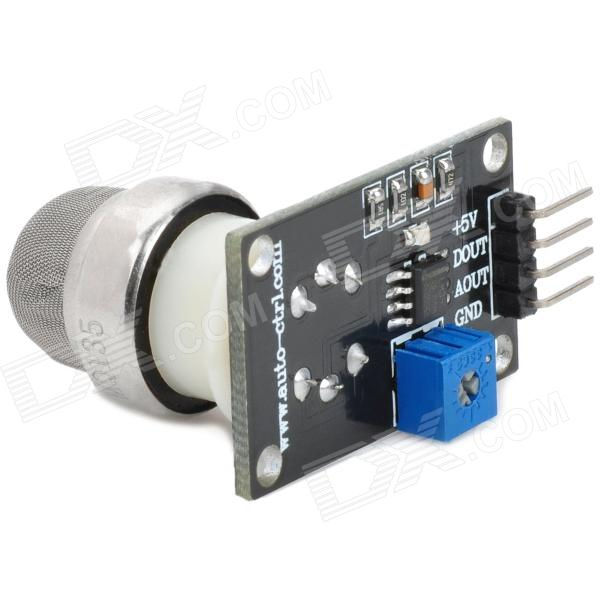
\includegraphics[width=0.7\textwidth]{./Figures/mq135.jpg}
                \caption{MQ135 Air Quality sensor}
                \label{fig:MQ135}
        \end{subfigure}%
        ~ %add desired spacing between images, e. g. ~, \quad, \qquad, \hfill etc.
          %(or a blank line to force the subfigure onto a new line)
        \begin{subfigure}[b]{0.3\textwidth}
                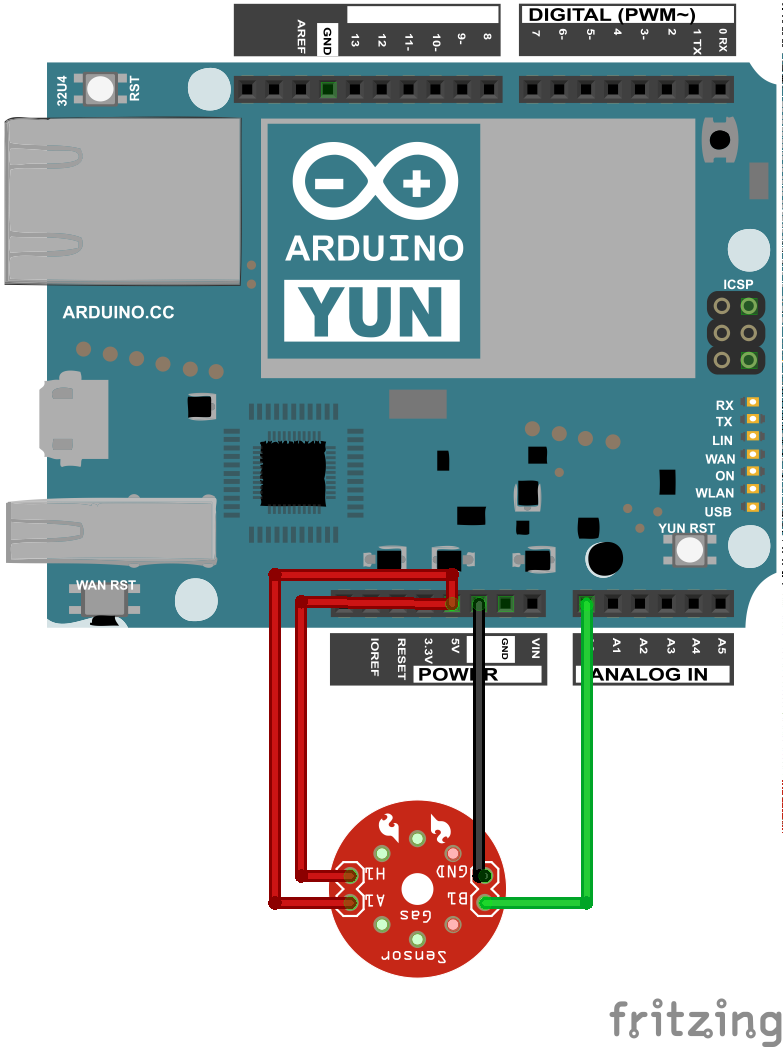
\includegraphics[width=\textwidth]{./Figures/Fritzing/GasSensor_bb.png}
                \caption{Gas Sensor Breadboard}
                \label{fig:GasSensor_bb}
        \end{subfigure}
        \rule{18em}{0.5pt}
        \caption{DHT11 sensor}\label{fig:DHT11sensor}
			\end{figure} 
      
      The Mq135 sensor reacts to the concentration of the following gases: NH3, NOx, alcohol, Benzene, smoke, CO2, etc.. \cite{mq135gassensor}.
      
    \subsection{BreadBoard with all the sensors}
      
      In the figure \ref{fig:AllSensors22_bb} is shown the final prototype with the DHT22 sensor, and in the figure \ref{fig:AllSensors11_bb} with the DHT11 sensor.
      
      \begin{figure}[!htbp]
          \centering
              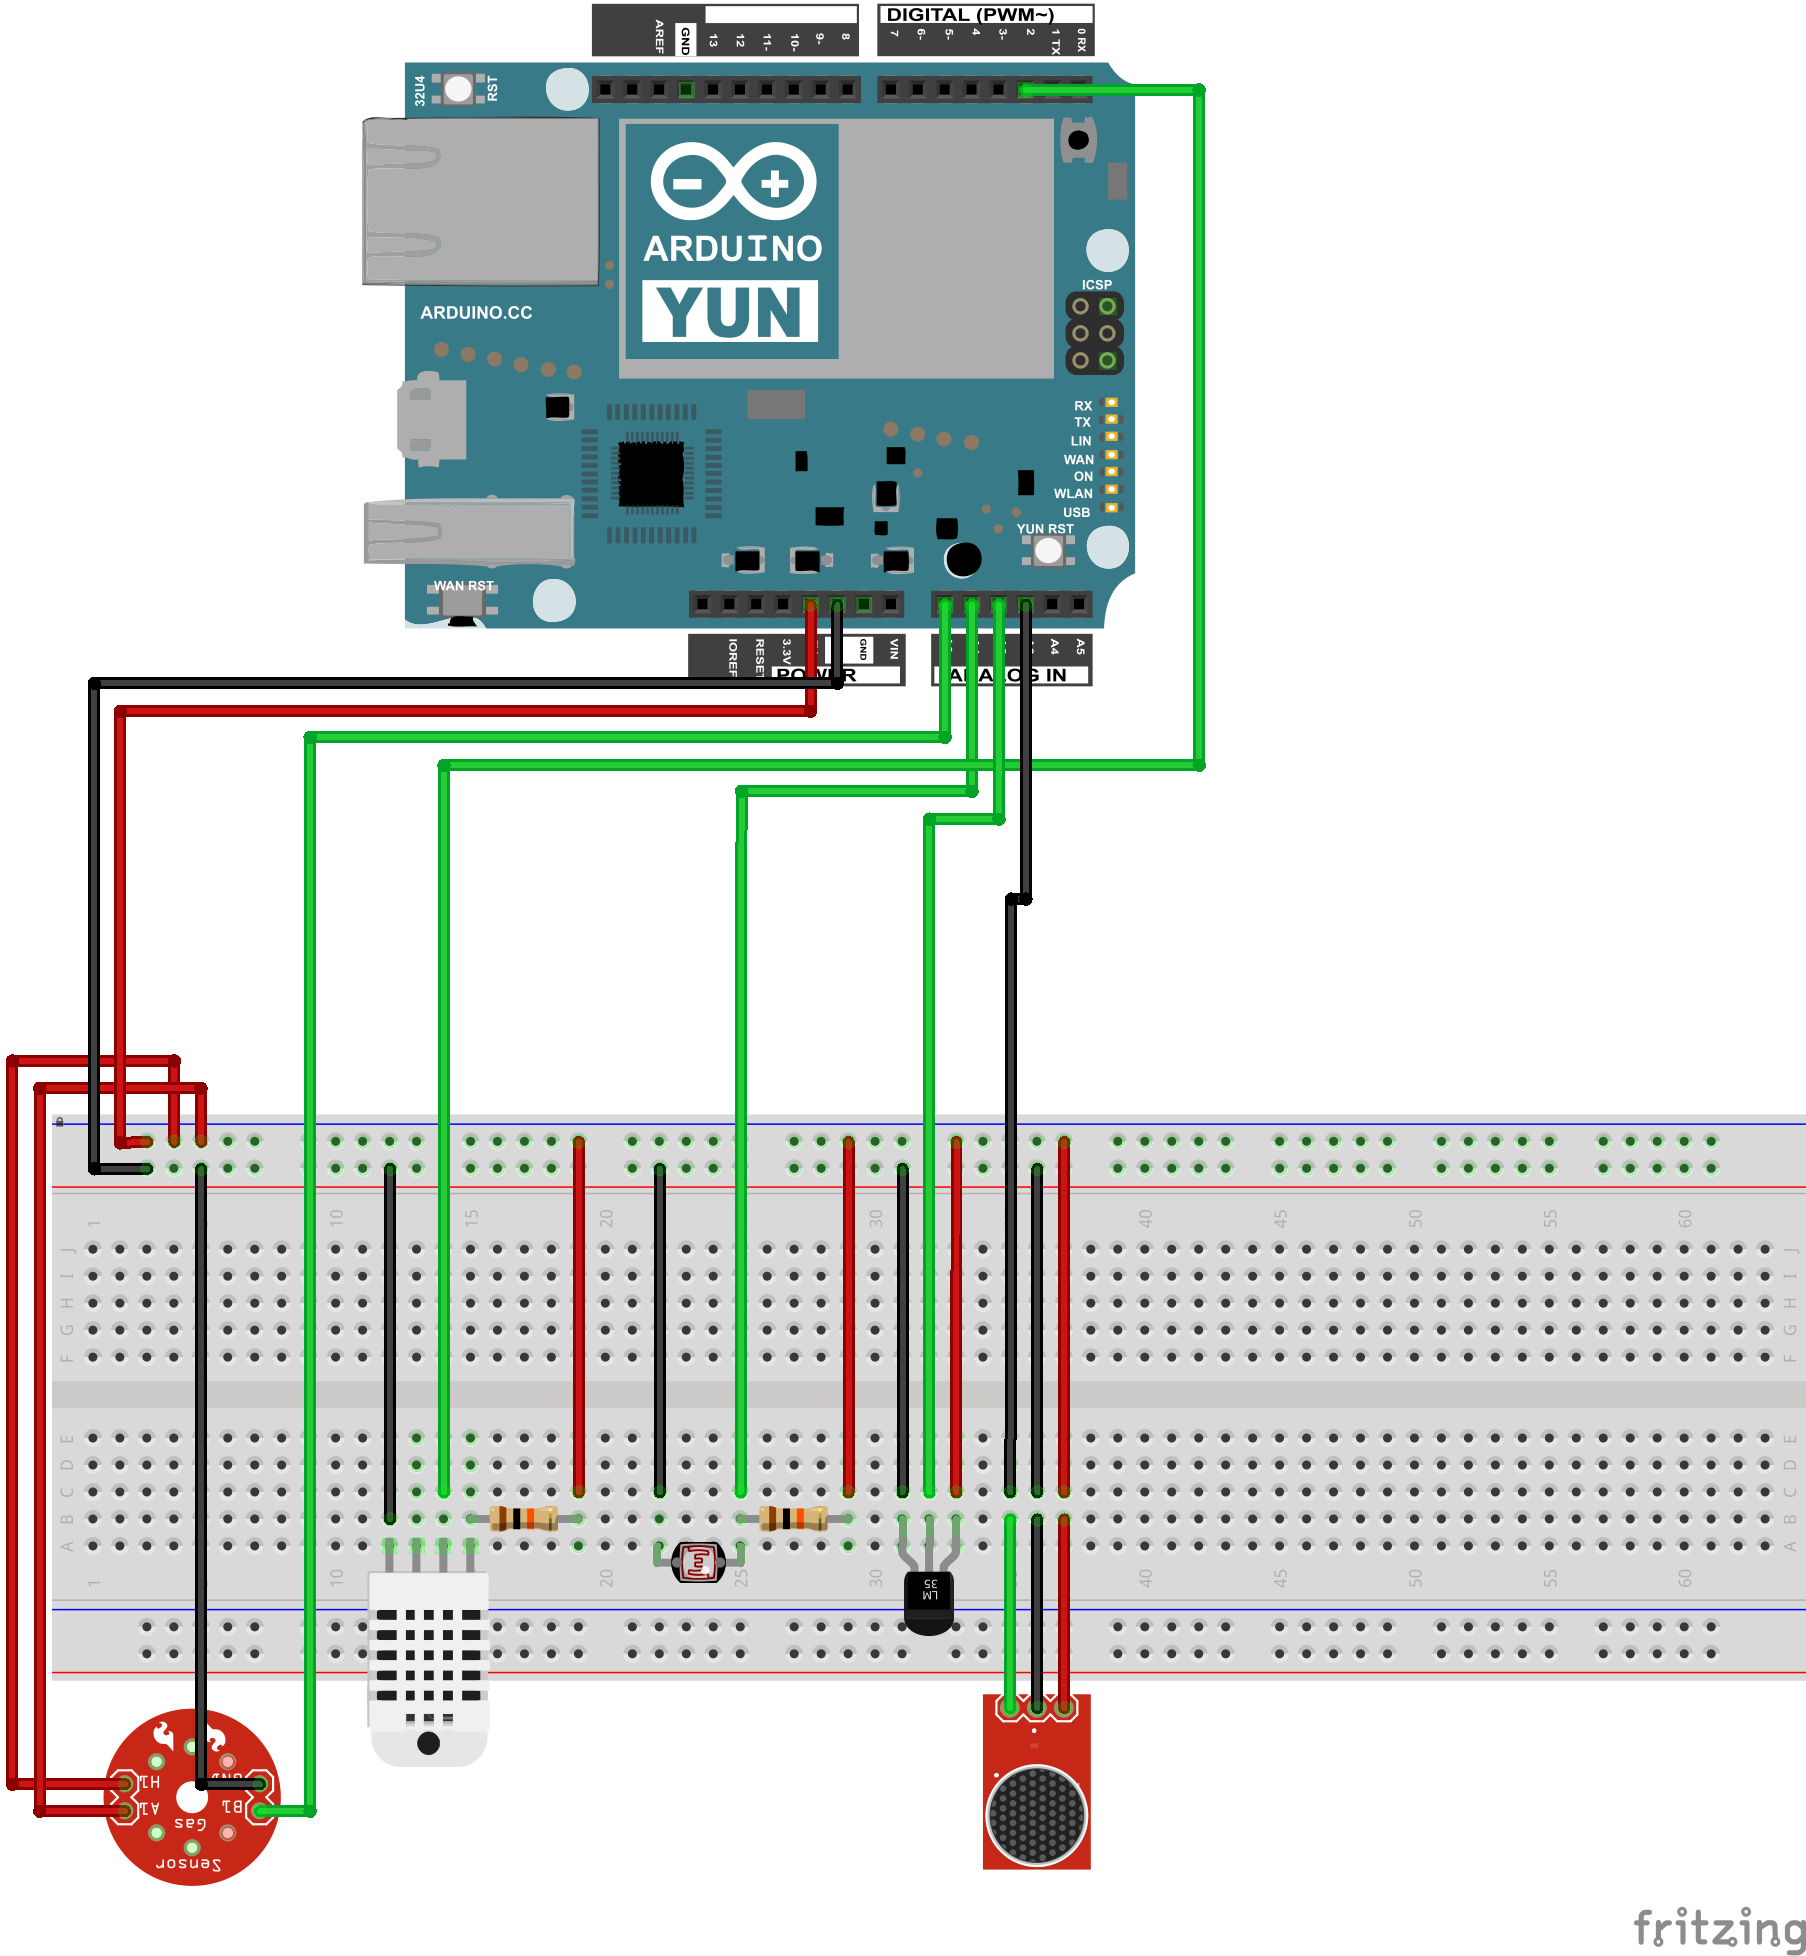
\includegraphics[scale=0.8]{./Figures/Fritzing/AllSensors22_bb.png}
              \rule{25em}{0.5pt}
          \caption[Sensor node Prototype with DHT22]{Sensor node Prototype with DHT22.}
          \label{fig:AllSensors22_bb}
      \end{figure}
      
      \begin{figure}[!htbp]
          \centering
              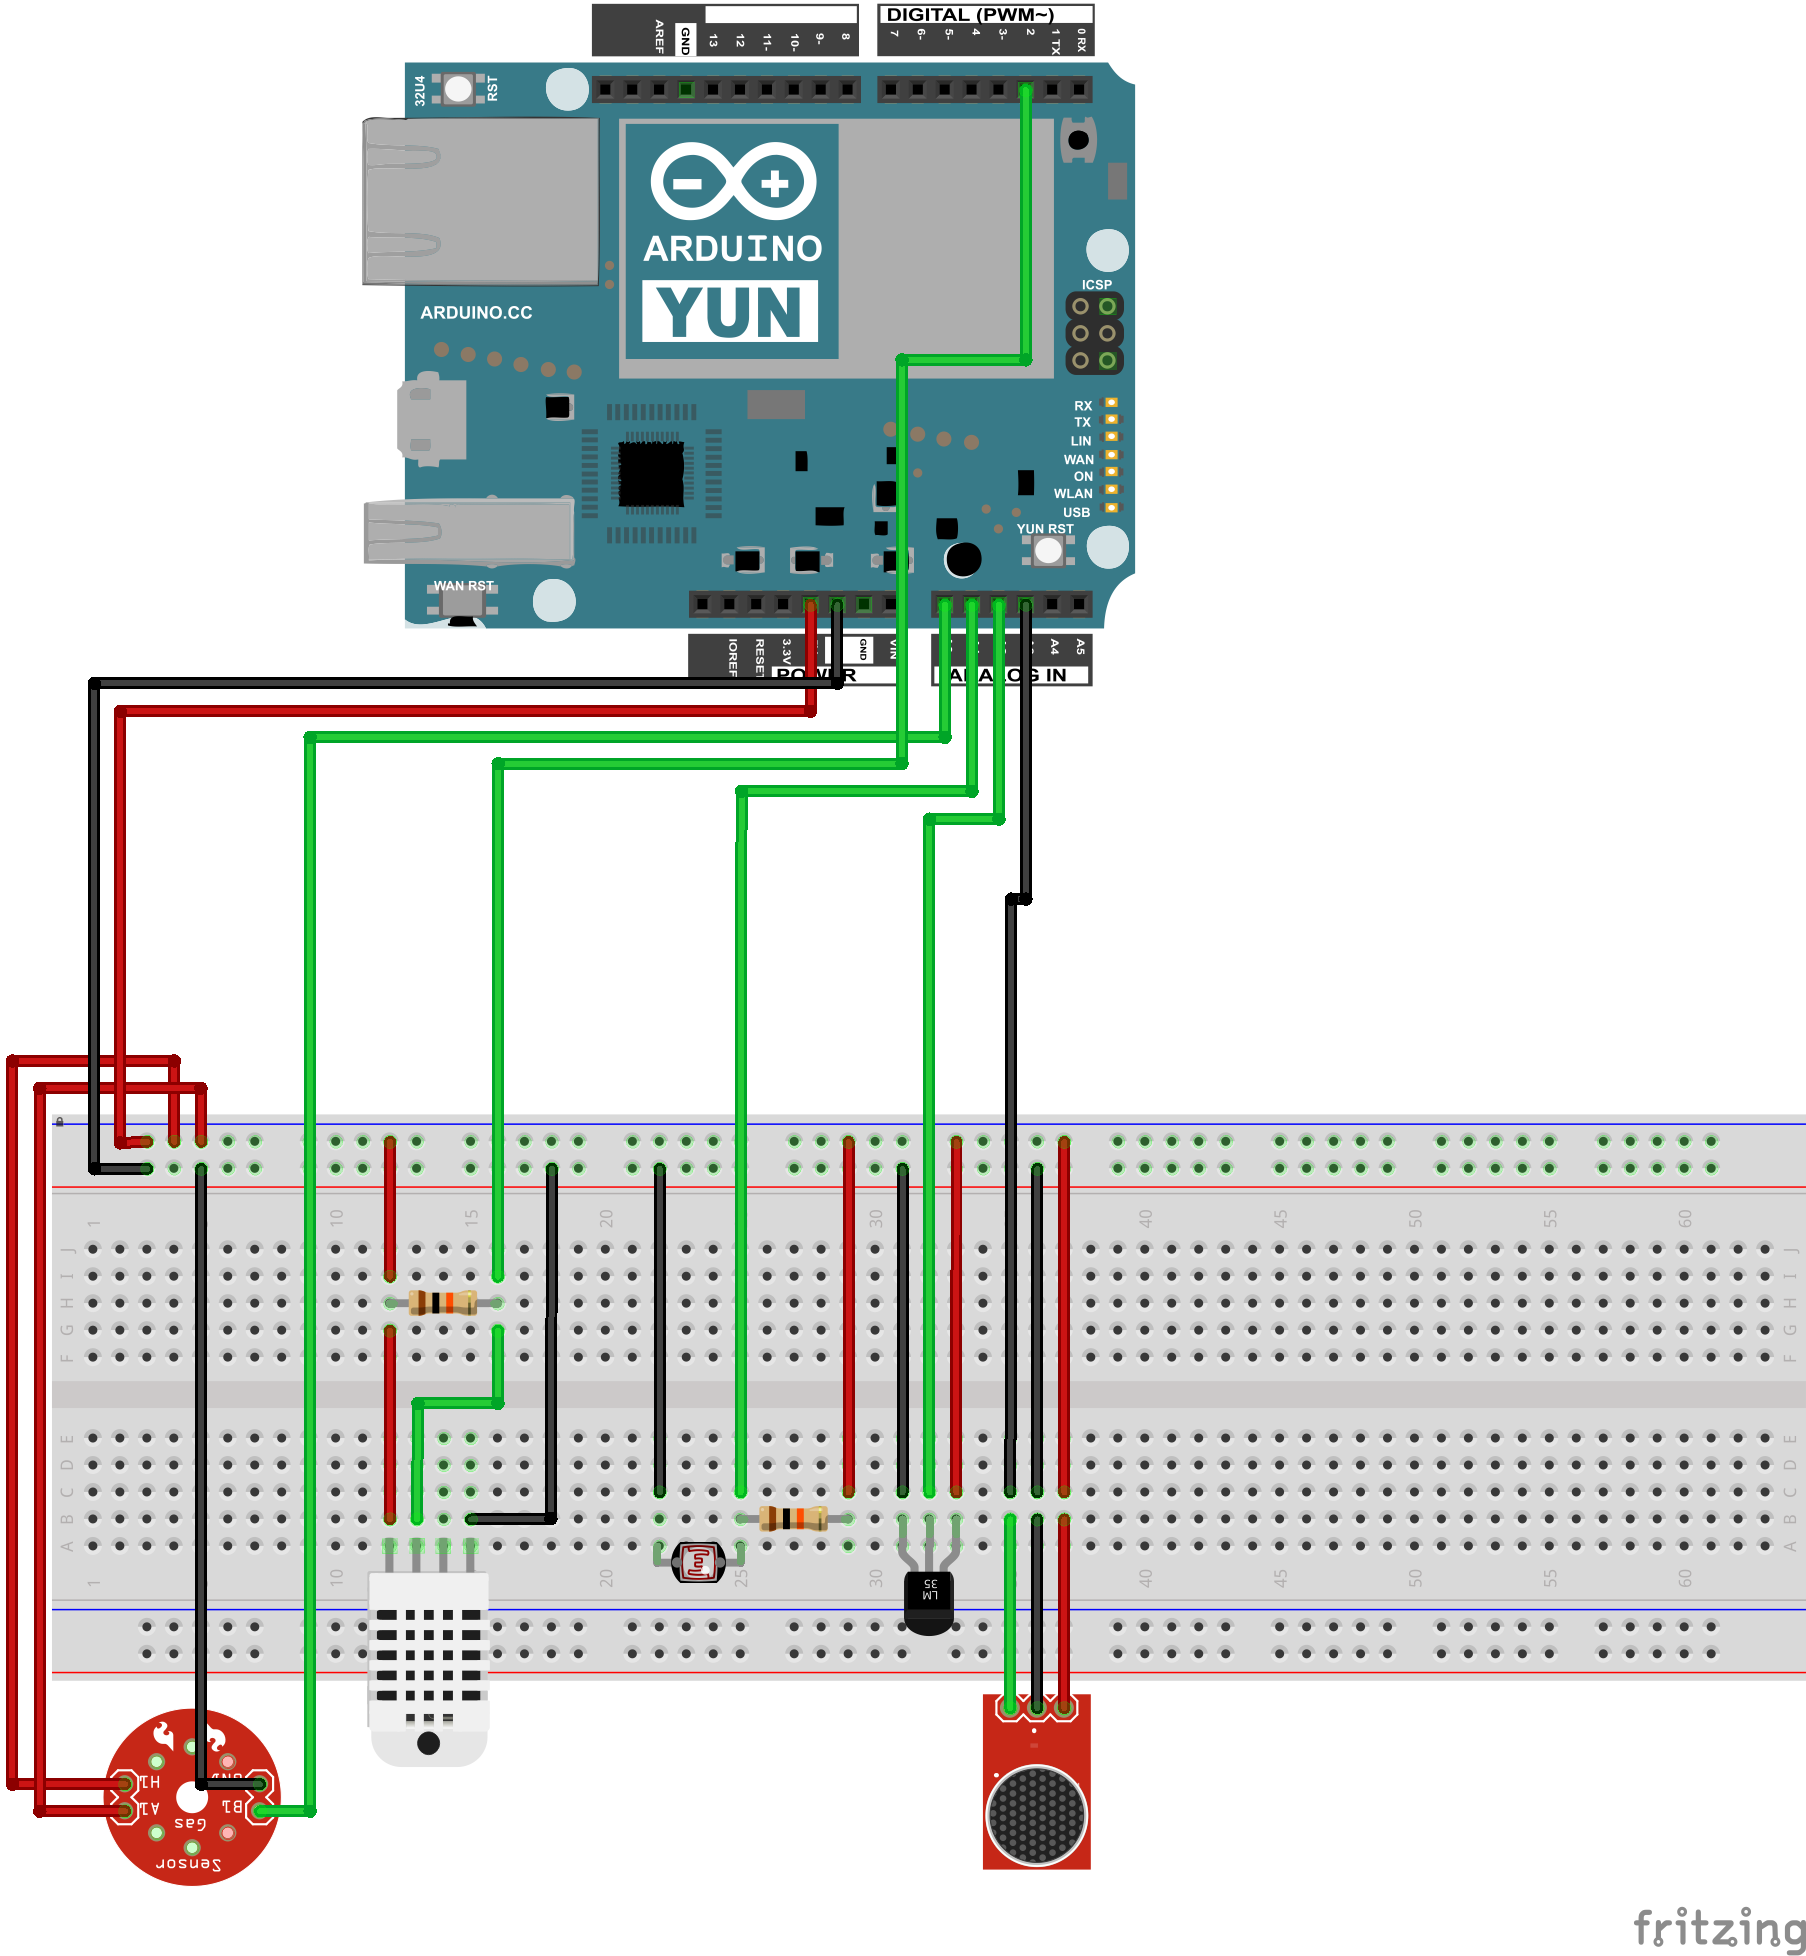
\includegraphics[scale=0.8]{./Figures/Fritzing/AllSensors11_bb.png}
              \rule{25em}{0.5pt}
          \caption[Sensor node Prototype with DHT11]{Sensor node Prototype with DHT11.}
          \label{fig:AllSensors11_bb}
      \end{figure}
    
  \section{Upload sensor data}
  
    A main part of the project is upload the data from the sensors to a platform so that everyone can access them.
    
    The GeoJSON message (Explained in section \ref{GeoJSON}) includes data from 5 sensors, which makes its size too large for the memory of the Arduino.
    For this type of operations is possible to run a script in the Linux environment through the bridge library\ref{fig:BridgeInShort}.
    
    This being the path that is followed, there are several options for developing this script, for example, programmed in Java, C / C + +, python, etc..

    Python has been used because of the following reasons: fast and perfect for prototyping programming, the code is shorter and therefore, easier to understand, and modular.
    
    \subsection{GeoJSON}
    \label{GeoJSON}
      A GeoJSON\footnote{\url{http://geojson.org/}} is a format for encoding a variety of geographic data structures. The GeoJSON that has been used is a collection of features, every feature contains a geometry object, in our case, a ``point'' with the longitud and latitud of the sensor node, and some properties required: ID, name, datasetID, datasetName, address, description, timestamp, value of the sensor, and unit.
      
      In the figure \ref{GeoJSON} it can be see an example of a GeoJSON message that is used in this project.
      \begin{figure}[htbp]
        \centering
            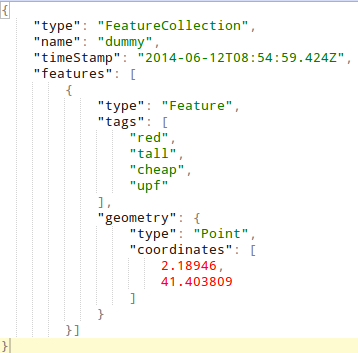
\includegraphics[scale=0.5]{./Figures/GeoJSON.png}
            \\
            \rule{15em}{0.5pt}
        \caption[GeoJSON message]{GeoJSON message.}
        \label{fig:GeoJSON}
      \end{figure}
    
  \section{Community network}
    Guifi \footnote{\url{https://www.guifi.net/}} is the network where the Arduino will be deployed, and the one providing the access to Opencities through the Internet.
    Guifi is a network created by people interested in building an open, free and neutral network infrastructure.
    
    Because of their philosophy of participation, Guifi is the perfect network for the deployment of this sensor nodes. Also their network is large enough to become a useful sensor network, as it can be seen in the figure \ref{fig:Guifimap}.
    \begin{figure}[htbp]
      \centering
          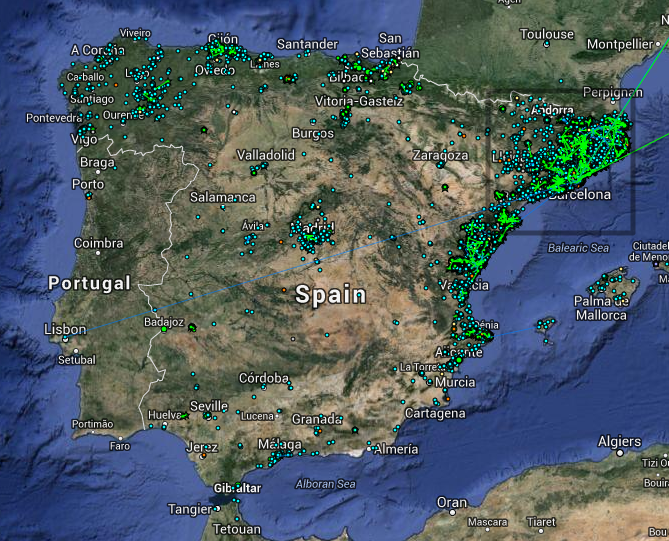
\includegraphics[scale=0.5]{./Figures/Guifimap.png}
          \rule{25em}{0.5pt}
      \caption[Guifi sensor map]{Guifi sensor map.}
      \label{fig:Guifimap}
    \end{figure}
    
  \section{Storage Resource Broker}  
    Opencities \cite{opencities} is the opendata services that has been chosen, for these reasons:
    \begin{itemize}
      \item The developers are at UPF, so the process of improving both projects (feedback, bug fixing, ...) can be fast and effective.
      \item Easy API to upload and download the data.
    \end{itemize}
    
    The role of Opencities is to be the intermediary between data creators and data users.
    In Opencities, the sensor data is uploaded into a dataset. Every user has an unique API key, and can create one or more datasets with a unique ID. 
    
  \section{Visualization platform}
    
    For the purpose of the sensor data visualization there are several options, in plain text, in a map, in graphics, etc. In this project a map is used to display the data. This can be done on a web page, in a mobile application, tablet application, etc.
    
    Since the goal of the application is that a user checks it for a small period of time, the best option is a mobile application. Additionally, almost everybody has an smart phone.
    
    There are three mobile operating system, iOS, Android, or Windows Phone. There is another option that is to developed the application in html5, javascript, and CSS, and then compile it with phonegap\footnote{\url{http://phonegap.com/}}, and that will build the application for the three operating systems. But it ended up being much more difficult than to create an application directly to an operating system, so the best choice is the one with more market share, to reach as many people as possible.  
      
    Android is a mobile operating system from Google, it runs on smartphones, and applications are programmed in Java. Java is a computer programming language that is object-oriented.    
    This application will be tested on a Sony Xperia Z1, with an Android 4.4.2.

\chapter{Bottom up sensor testbed}
\label{Chapter4}

  This chapter is focused on the process followed to finish the project, which has two main parts, the software to collect and send the data and the Android application to show it. A scheme of the project is shown in Figure \ref{fig:reportGeneralView}.
  
  \begin{figure}[htbp]
    \centering
        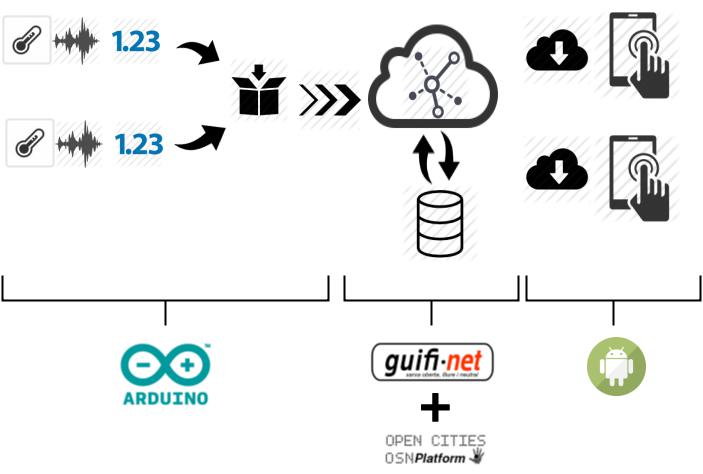
\includegraphics[scale=0.5]{./Figures/reportGeneralView.jpg}
        \rule{25em}{0.5pt}
    \caption[reportGeneralView]{reportGeneralView.}
    \label{fig:reportGeneralView}
  \end{figure}
  
  \section{Arduino Development}
    
    Two scripts has been needed, one to collect the data, and other to send it. This is because the memory to run an Arduino sketch is very low, and the creation of the GeoJSON message to Opencities is too big with respect to the available memory. That is why a python script has been used, called first by the Arduino sketch.
    
    The Arduino sketch is responsible of collecting the data, write it down in a logData file, and call the python script with the collected values and an unique ID. Finally the python script has to create a GeoJSON and send it to Opencities.
    
    \subsection{Collect sensor data}
    
      To collect almost all the data the skecth does not need to include external libraries, except for the humidity sensors (DHT22 and DHT11)\footnote{\url{https://github.com/adafruit/DHT-sensor-library}}.
      
      The following libraries were needed to develope the code: FileIO, Process library, Bridge.
      
      The Arduino sketch is code in a very simple way, the setup function will initialize the Bridge library to communicate with the Linux environment, the Serial library for debugging purposes, and the FileSystem to log the process, and the loop function. The loop will call three functions: readSensors, readFile, and executePythonScript.
      
      \begin{itemize}
        \item {\bf readSensors:} It call 5 different functions to read every sensor, the reason for doing a separate function is to make the code more clear.
        \item {\bf readFile:} This function logs the process, saves the ID of the message, the sensor values, and a timestamp.
        \item {\bf executePythonScript:} The script in python located in the SD card is in charge to create the GeoJSON with all the sensor data and upload it to Opencities. This script is called by the Arduino sketch.
      \end{itemize}
      
      The figure \ref{fig:Arduino sketch Flow Chart} explain how the Arduino sketch works.\\
      
      \begin{figure}[htbp]
      \centering

      \begin{tikzpicture}[node distance=2cm]

        \node (bridge) [startstop] {Initialize Bridge};
        \node (Serial) [process, below of=bridge] {Initialize Serial};
        \node (FileSystem) [process, below of=Serial] {Initialize FileSystem};
        \node (ReadSensors) [process, below of=FileSystem] {Read Sensors};
        \node (ReadFile) [process, below of=ReadSensors] {Read \& Write File};
        \node (delay) [process, right of=ReadFile, xshift=2cm] {Delay of 48 seconds};
        \node (ExecutePython) [process, below of=ReadFile] {Execute Python Script};
        
        \draw [arrow] (bridge) -- (Serial);
        \draw [arrow] (Serial) -- (FileSystem);
        \draw [arrow] (FileSystem) -- (ReadSensors);
        \draw [arrow] (ReadSensors) -- (ReadFile);
        \draw [arrow] (ReadFile) -- (ExecutePython);
        \draw [arrow] (ExecutePython) -| (delay);
        \draw [arrow] (delay) |- (ReadSensors);

      \end{tikzpicture}
      \rule{35em}{0.5pt}
      \caption[Arduino sketch Flow Chart]{Arduino sketch Flow Chart.}
      \label{fig:Arduino sketch Flow Chart}
      \end{figure}
    
    \subsection{Communication with Opencities}
    
      To communicate with Opencities it is necessary to create an acount, and a dataset to store the sensor data. At the end, the user has an API key and a dataset ID, the required information to upload and download data. 
      
      The communication with Opencities is done by means of a python script. This are the packages needed into the Linux environment of the Arduino: distribute, python-openssl, geojson, geopy, and httplib2.
      
      The python script has three process, first it stores all the sensor data pass by the Arduino sketch into a class. Then it creates a GeoJSON message with all the data, and all the parameters needed to upload it into Opencities. Finally upload the GeoJSON message.
      
      With all this libraries the script can communicate with Opencities and store the sensor data collected by the Arduino. The \ref{fig:Python Script Flow Chart} figure explains how the python script works.\\
      
      \begin{figure}[!htbp]
      \centering

      \begin{tikzpicture}[node distance=2cm]      
        
        \node (start) [startstop] {Called by the Arduino};
        \node (CorrectUsage) [decision, below of=start, yshift=-2cm] {Is the usage correct};
        \node (collectdata) [process, below of=CorrectUsage, yshift=-2cm] {Store the arguments as sensor data};
        \node (ShowCorrectWay) [process, right of=CorrectUsage, xshift=4cm] {Show the correct usage};
        \node (StopUsage) [startstop, right of=ShowCorrectWay, xshift=2cm] {Stop};
        \node (CreateGeoJSON) [process, below of=collectdata] {Create GeoJSON};
        \node (PostOpencities) [process, below of=CreateGeoJSON] {POST in Opencities};
        \node (stop) [startstop, below of=PostOpencities] {Stop};
        
        \draw [arrow] (start) -- (CorrectUsage);
        \draw [arrow] (CorrectUsage) -- node[anchor=east] {yes} (collectdata);
        \draw [arrow] (CorrectUsage) -- node[anchor=south] {no} (ShowCorrectWay);
        \draw [arrow] (ShowCorrectWay) -- (StopUsage);
        \draw [arrow] (collectdata) -- (CreateGeoJSON);
        \draw [arrow] (CreateGeoJSON) -- (PostOpencities);
        \draw [arrow] (PostOpencities) -- (stop);
        

      \end{tikzpicture}
      \rule{35em}{0.5pt}
      \caption[Python Script Flow Chart]{Python Script Flow Chart.}
      \label{fig:Python Script Flow Chart}
      \end{figure}
      
  \section{Android app}
  
    \subsection{Summary}

      To make easy to see the results of the testbed, an Android application has been developed which shows the sensor data in a map. The application shows the data in two ways, with markers that show the actual value in that point, and also with heatmap points, the larger the value, the more intense the red will be. This can be seen in figure \ref{fig:AppScreenshots}.
      
    \subsection{Interface}
      The application interface is a unique map view where the user can zoom to a limit, go to his location, and use the top buttons to change the sensor read. From left to right, the first button is the Marker button, the user decides whether the markers are displayed or not, and the next buttons refer to the type of sensor data to show as markers and/or as heatmap points (Temperature, Humidity, Noise, Light, and Air Quality).
      If the Marker button is checked, the user can click on the marker in the map and it will show the value of the temperature, humidity,... and the unit (Figure \ref{fig:AppScreenshots}).
      \begin{figure}
        \centering
        \begin{subfigure}[b]{0.3\textwidth}
                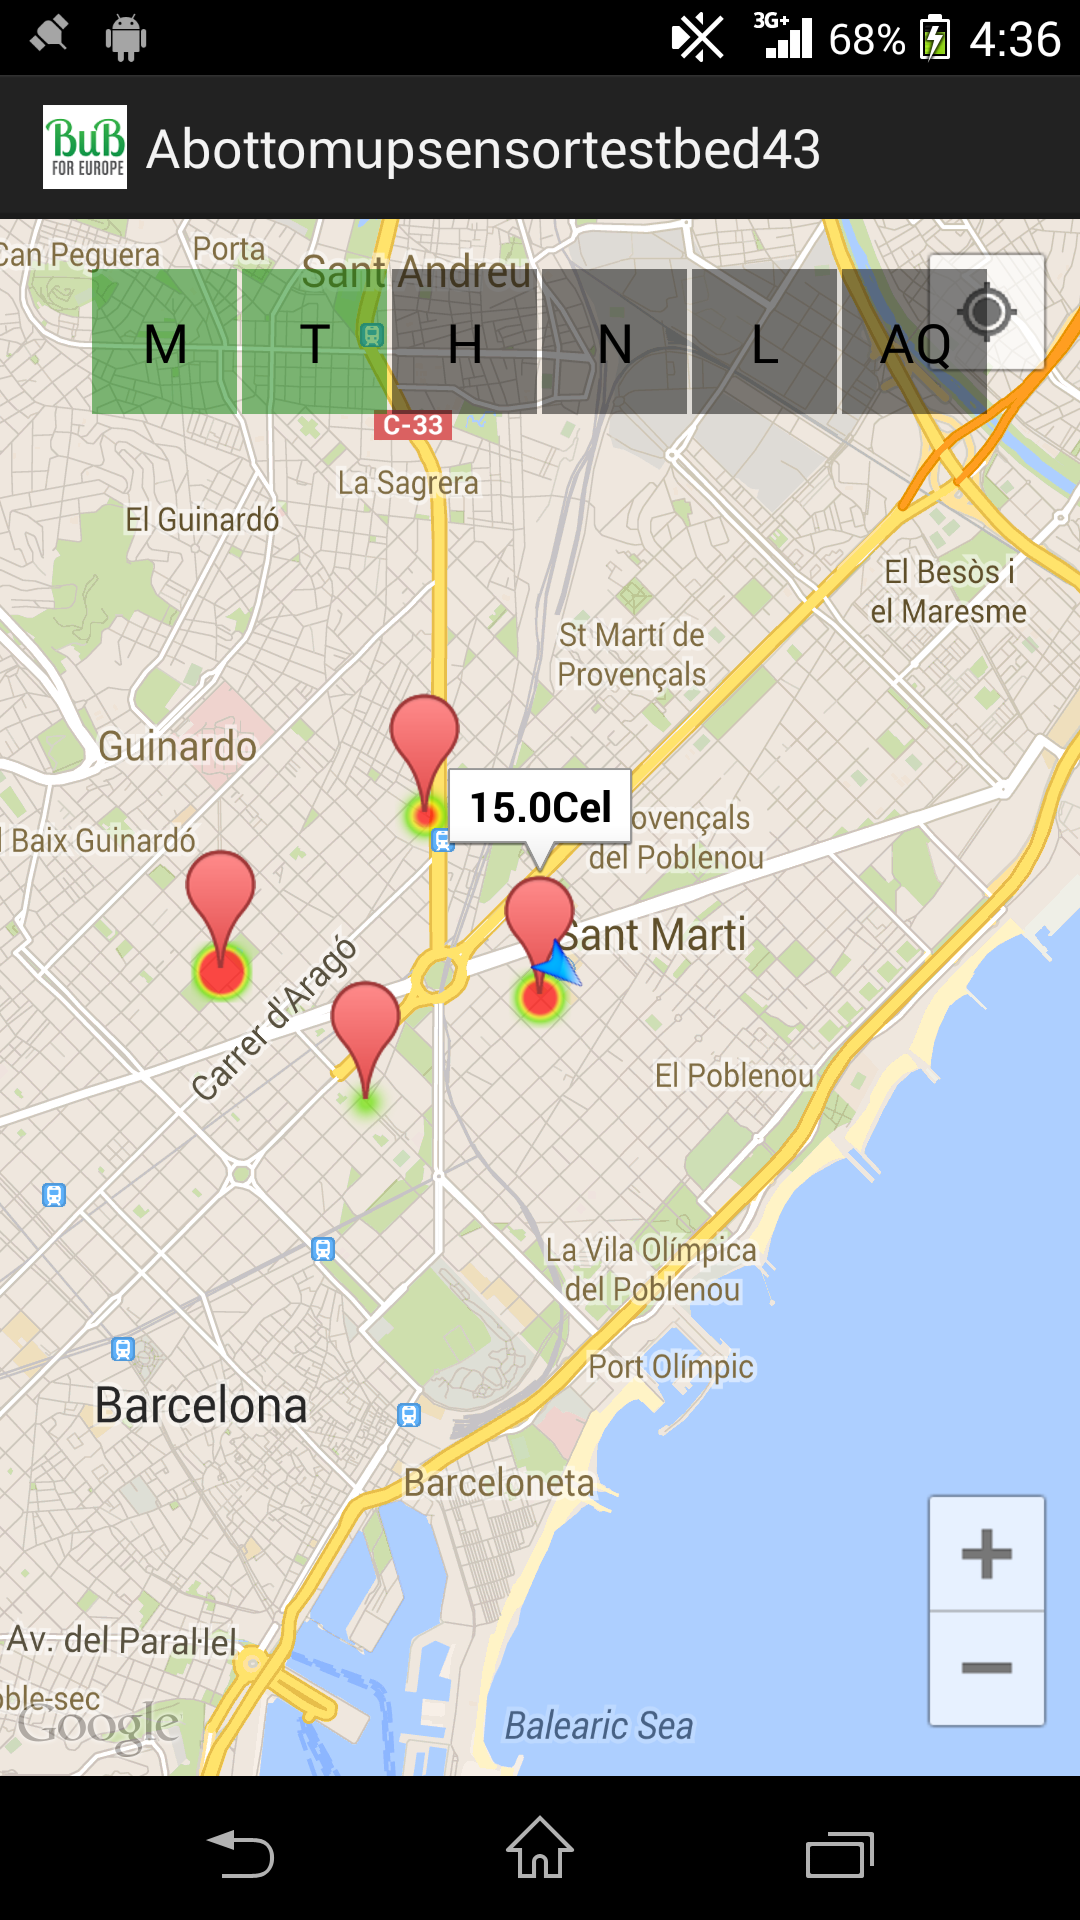
\includegraphics[width=\textwidth]{./Figures/App_Screenshot_1.png}
                \label{fig:App_Screenshot_1}
        \end{subfigure}%
        ~ %add desired spacing between images, e. g. ~, \quad, \qquad, \hfill etc.
          %(or a blank line to force the subfigure onto a new line)
        \begin{subfigure}[b]{0.3\textwidth}
                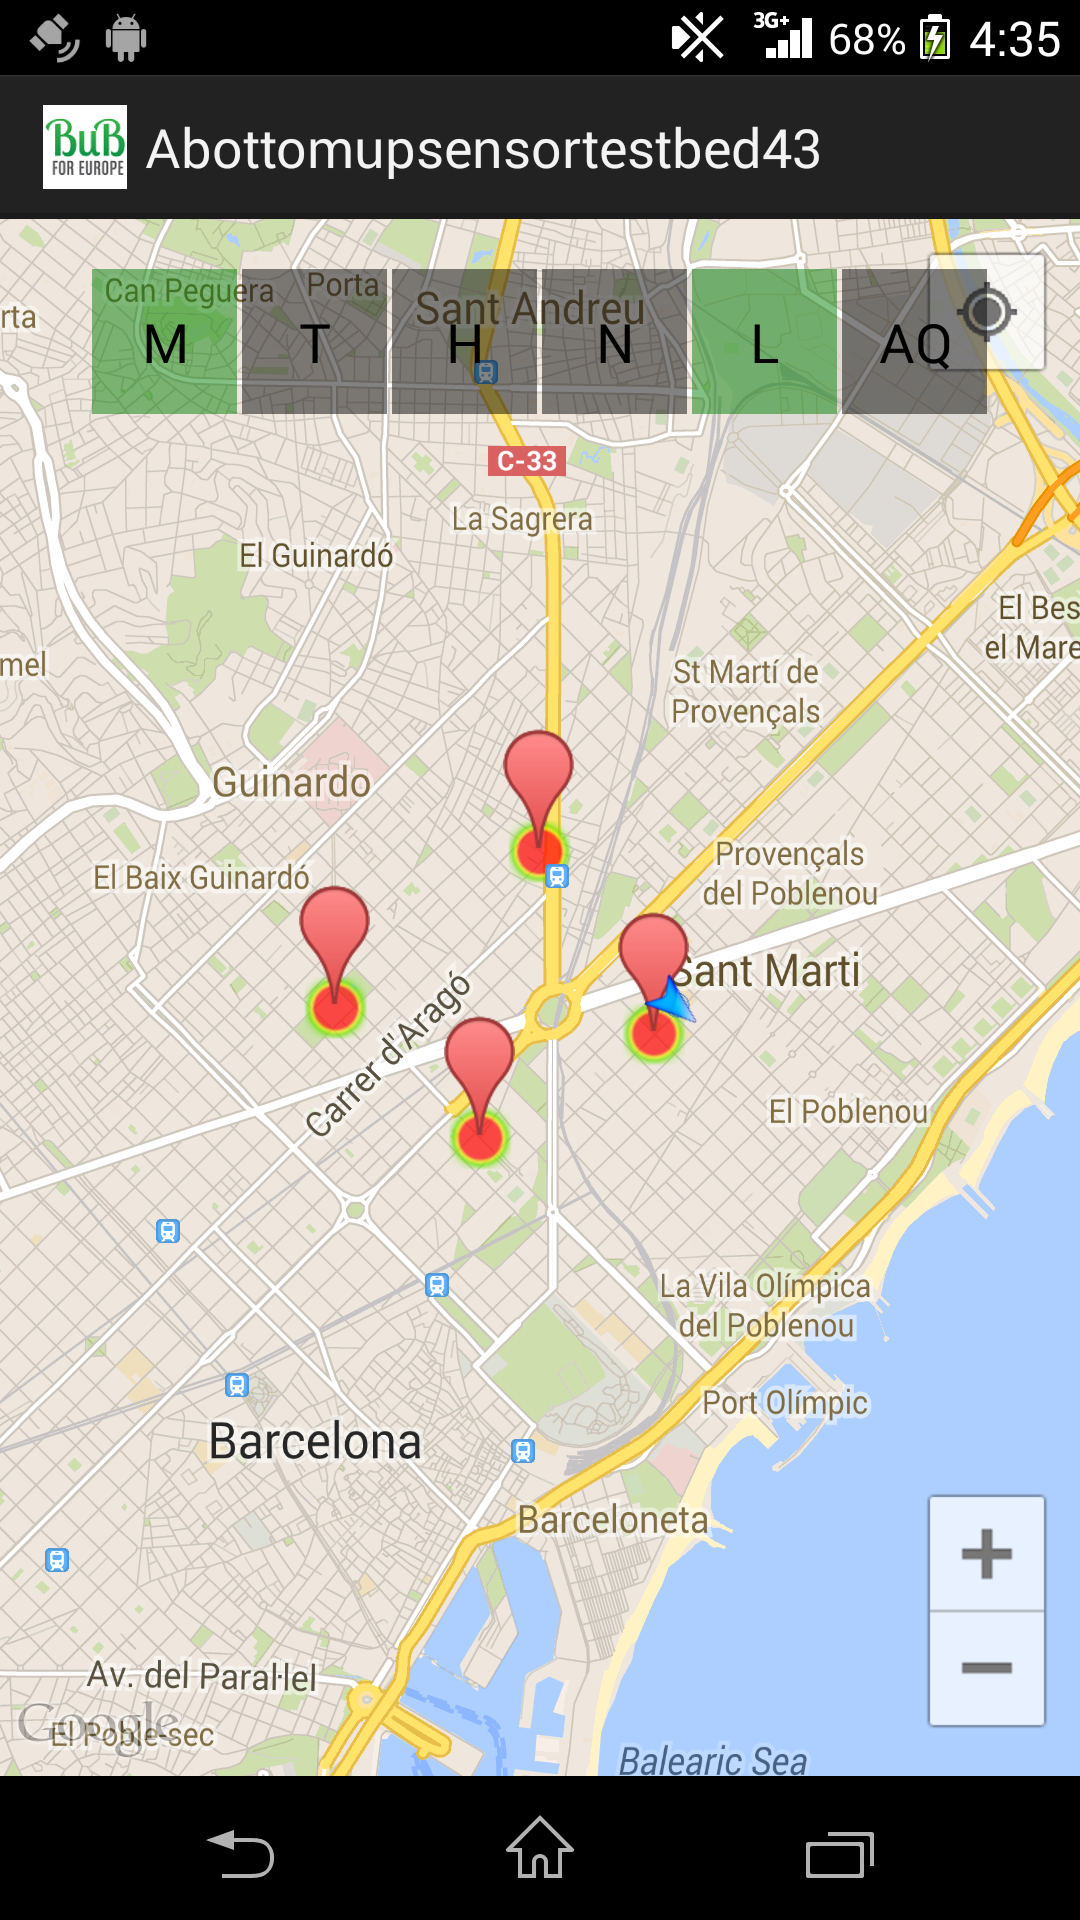
\includegraphics[width=\textwidth]{./Figures/App_Screenshot_3.png}
                \label{fig:App_Screenshot_2}
        \end{subfigure}
        \rule{18em}{0.5pt}
        \caption{App Screenshots}\label{fig:AppScreenshots}
\end{figure}
      
    \subsection{Code}
      First of all, to create this application the Google Maps Android API v2\footnote{\url{https://developers.google.com/maps/documentation/android/}} for the map view, and the Google Maps Android API utility library\footnote{\url{http://googlemaps.github.io/android-maps-utils/}} for the heatmaps are needed.
      
      In this application each class has a defined function, starting with MainActivity, which is the one that intialize the other clases, calls all the functions needed in the other classes to get the application started.
      
      It also has all the code to interact with the interface. For example, if the user clicks on the marker button, this class has to call all the necessary functions and display all the markers into the map.
      
      Next comes the dataBase class, which, as the name suggest, is the class that stores and processes the data downloaded from Opencities. This is a Singleton class, which means that there will only be one instance of this class and any instance of any class could access to the data stored on it.
      
      To stored the data from Opencities, there has been created a set of classes equivalent with the GeoJSON message downloaded to avoid confusion. At the end, the data is stored in features, which is composed primarly of Geometry and Properties.
      
      Then a class called HttpAsyncTask that handles the communication with Opencities and, using an instance of dataBase, stores the downloaded data.
      
      Finally, a GPSTracker class is responsible for obtaining user location to place the map on the user location, because it will be the place that the users want to see.
           
      A reduce class diagram can be seen in the figure \ref{fig:ClassDiagram}.
      
      \begin{figure}[htbp]
        \centering
          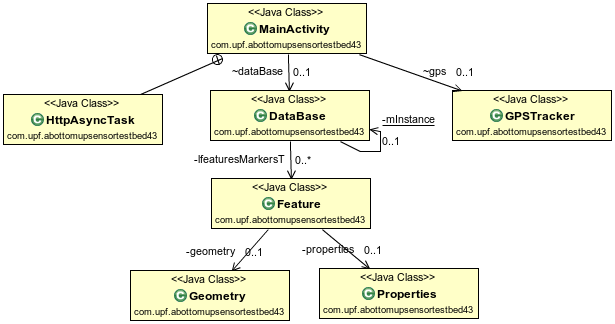
\includegraphics[page=1,scale=0.8]{./Figures/SmallClassDiagram.png}
        \rule{20em}{0.5pt}
        \caption[Reduce Class Diagram of the Android App]{Reduce Class Diagram of the Android App.}
        \label{fig:ClassDiagram}
      \end{figure}
      
      The explanation of the code is in the flow chart \ref{fig:Android App Flow Chart}.
      
      \begin{figure}[!htbp]
      \centering

      \begin{tikzpicture}[node distance=1cm]      
        
        \node (start) [startstop] {Initialize Google Map};
        \node (zoomlimit) [process, below of=start, yshift=-0.5cm] {Set zoom limit};
        \node (InitializeButtons) [process, below of=zoomlimit, yshift=-0.5cm] {Initialize all the Buttons and listeners};
        \node (GetCurrentLocation) [process, below of=InitializeButtons, yshift=-1cm] {Get Current Location using GPSTracker};
        \node (CallOpendata) [process, below of=GetCurrentLocation, yshift=-1cm] {Call OpenData, and parse the JSON};
        \node (CreateFeaturesByCoordinates) [process, below of=CallOpendata, yshift=-2cm] {Create a hashmap with all the features with the  coordinates as key, and a list of features for every key};
        \node (addMarkers) [process, below of=CreateFeaturesByCoordinates, yshift=-2cm] {Save only the latest features for every coordinate};
        \node (addHeatMapAndaddMakers2) [process, below of=addMarkers, yshift=-1.5cm] {Show the markers or heatmap points of a type of data};
        
        \draw [arrow] (start) -- (zoomlimit);
        \draw [arrow] (zoomlimit) -- (InitializeButtons);
        \draw [arrow] (InitializeButtons) -- (GetCurrentLocation);
        \draw [arrow] (GetCurrentLocation) -- (CallOpendata);
        \draw [arrow] (CallOpendata) -- (CreateFeaturesByCoordinates);
        \draw [arrow] (CreateFeaturesByCoordinates) -- (addMarkers);
        \draw [arrow] (addMarkers) -- (addHeatMapAndaddMakers2);
        

      \end{tikzpicture}
      \rule{35em}{0.5pt}
      \caption[Android App Flow Chart]{Android App Flow Chart.}
      \label{fig:Android App Flow Chart}
      \end{figure}

	\section{Repository}
		All the code, report, figures, etc has been stored in a public repository\footnote{\url{https://github.com/SergioAlmendros/A-bottom-up-sensor-testbed}}, so anyone could see it, downloaded a copy, and change it if necessary.
		
		In the figure \ref{fig:repository} it has been explained how the repository is distributed, each folder representes part of the process that has been done on this project.
		
		\begin{figure}[htbp]
			\centering
				  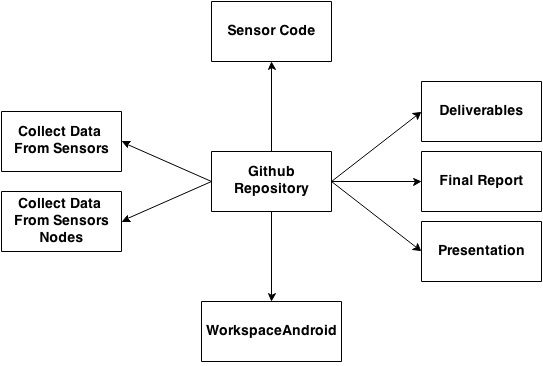
\includegraphics[scale=0.6]{./Figures/repository.png}
				  \rule{25em}{0.5pt}
			\caption[Github Repository]{Github Repository.}
			\label{fig:repository}
		\end{figure} 
		
		The most important folders are:
		\begin{itemize}
			\item {\bf Sensor Code:} Where has been stored the code that go into the Arduino (Arduino sketch and python script).
			\item {\bf WorkspaceAndroid:} This folder has been used as workspace for the developing of the mobile application using the IDE (Integrated Development Environment) Eclipse.
			\item {\bf Final Report:} Is where it has been documenting the project and has been written in latex, a system for the creation of technical and scientific documentation.
		\end{itemize}
		
		The less important folders are:
		\begin{itemize}
			\item {\bf Collect Data From Sensors:} Here has been stored the code to get the value of each sensor separately, in case someone wants to use only one of the sensors and dows not want to read the full code.
			\item {\bf Collect Data From Sensors Nodes:} Using the logData files that have been created during the testbed and an octave script that has been developped to read this data and display it in graphs.
			\item {\bf Deliverables:} In this folder it has been stored the initial documentation of the project.
			\item {\bf Presentation:} Finally, here is the slide presentation that has been made to explain the project, also written in latex.
		\end{itemize}
		
		During all the project there have been constant uploads of new information to the repository, as it was evolving.


\chapter{Testbed Deployment and Results}
\label{Chapter5}

  In this chapter the procedure to deploy a testbed had been explained step by step.
  
  In the figure \ref{fig:TestBed_Prototype} there is a photograph of the prototype used in this testbed. It is composed of an Arduino YUN, a microSD card, a breadboard, and all the sensor connected (temperature, humidity, noise, light, and gas).
  
  \begin{figure}[htbp]
      \centering
          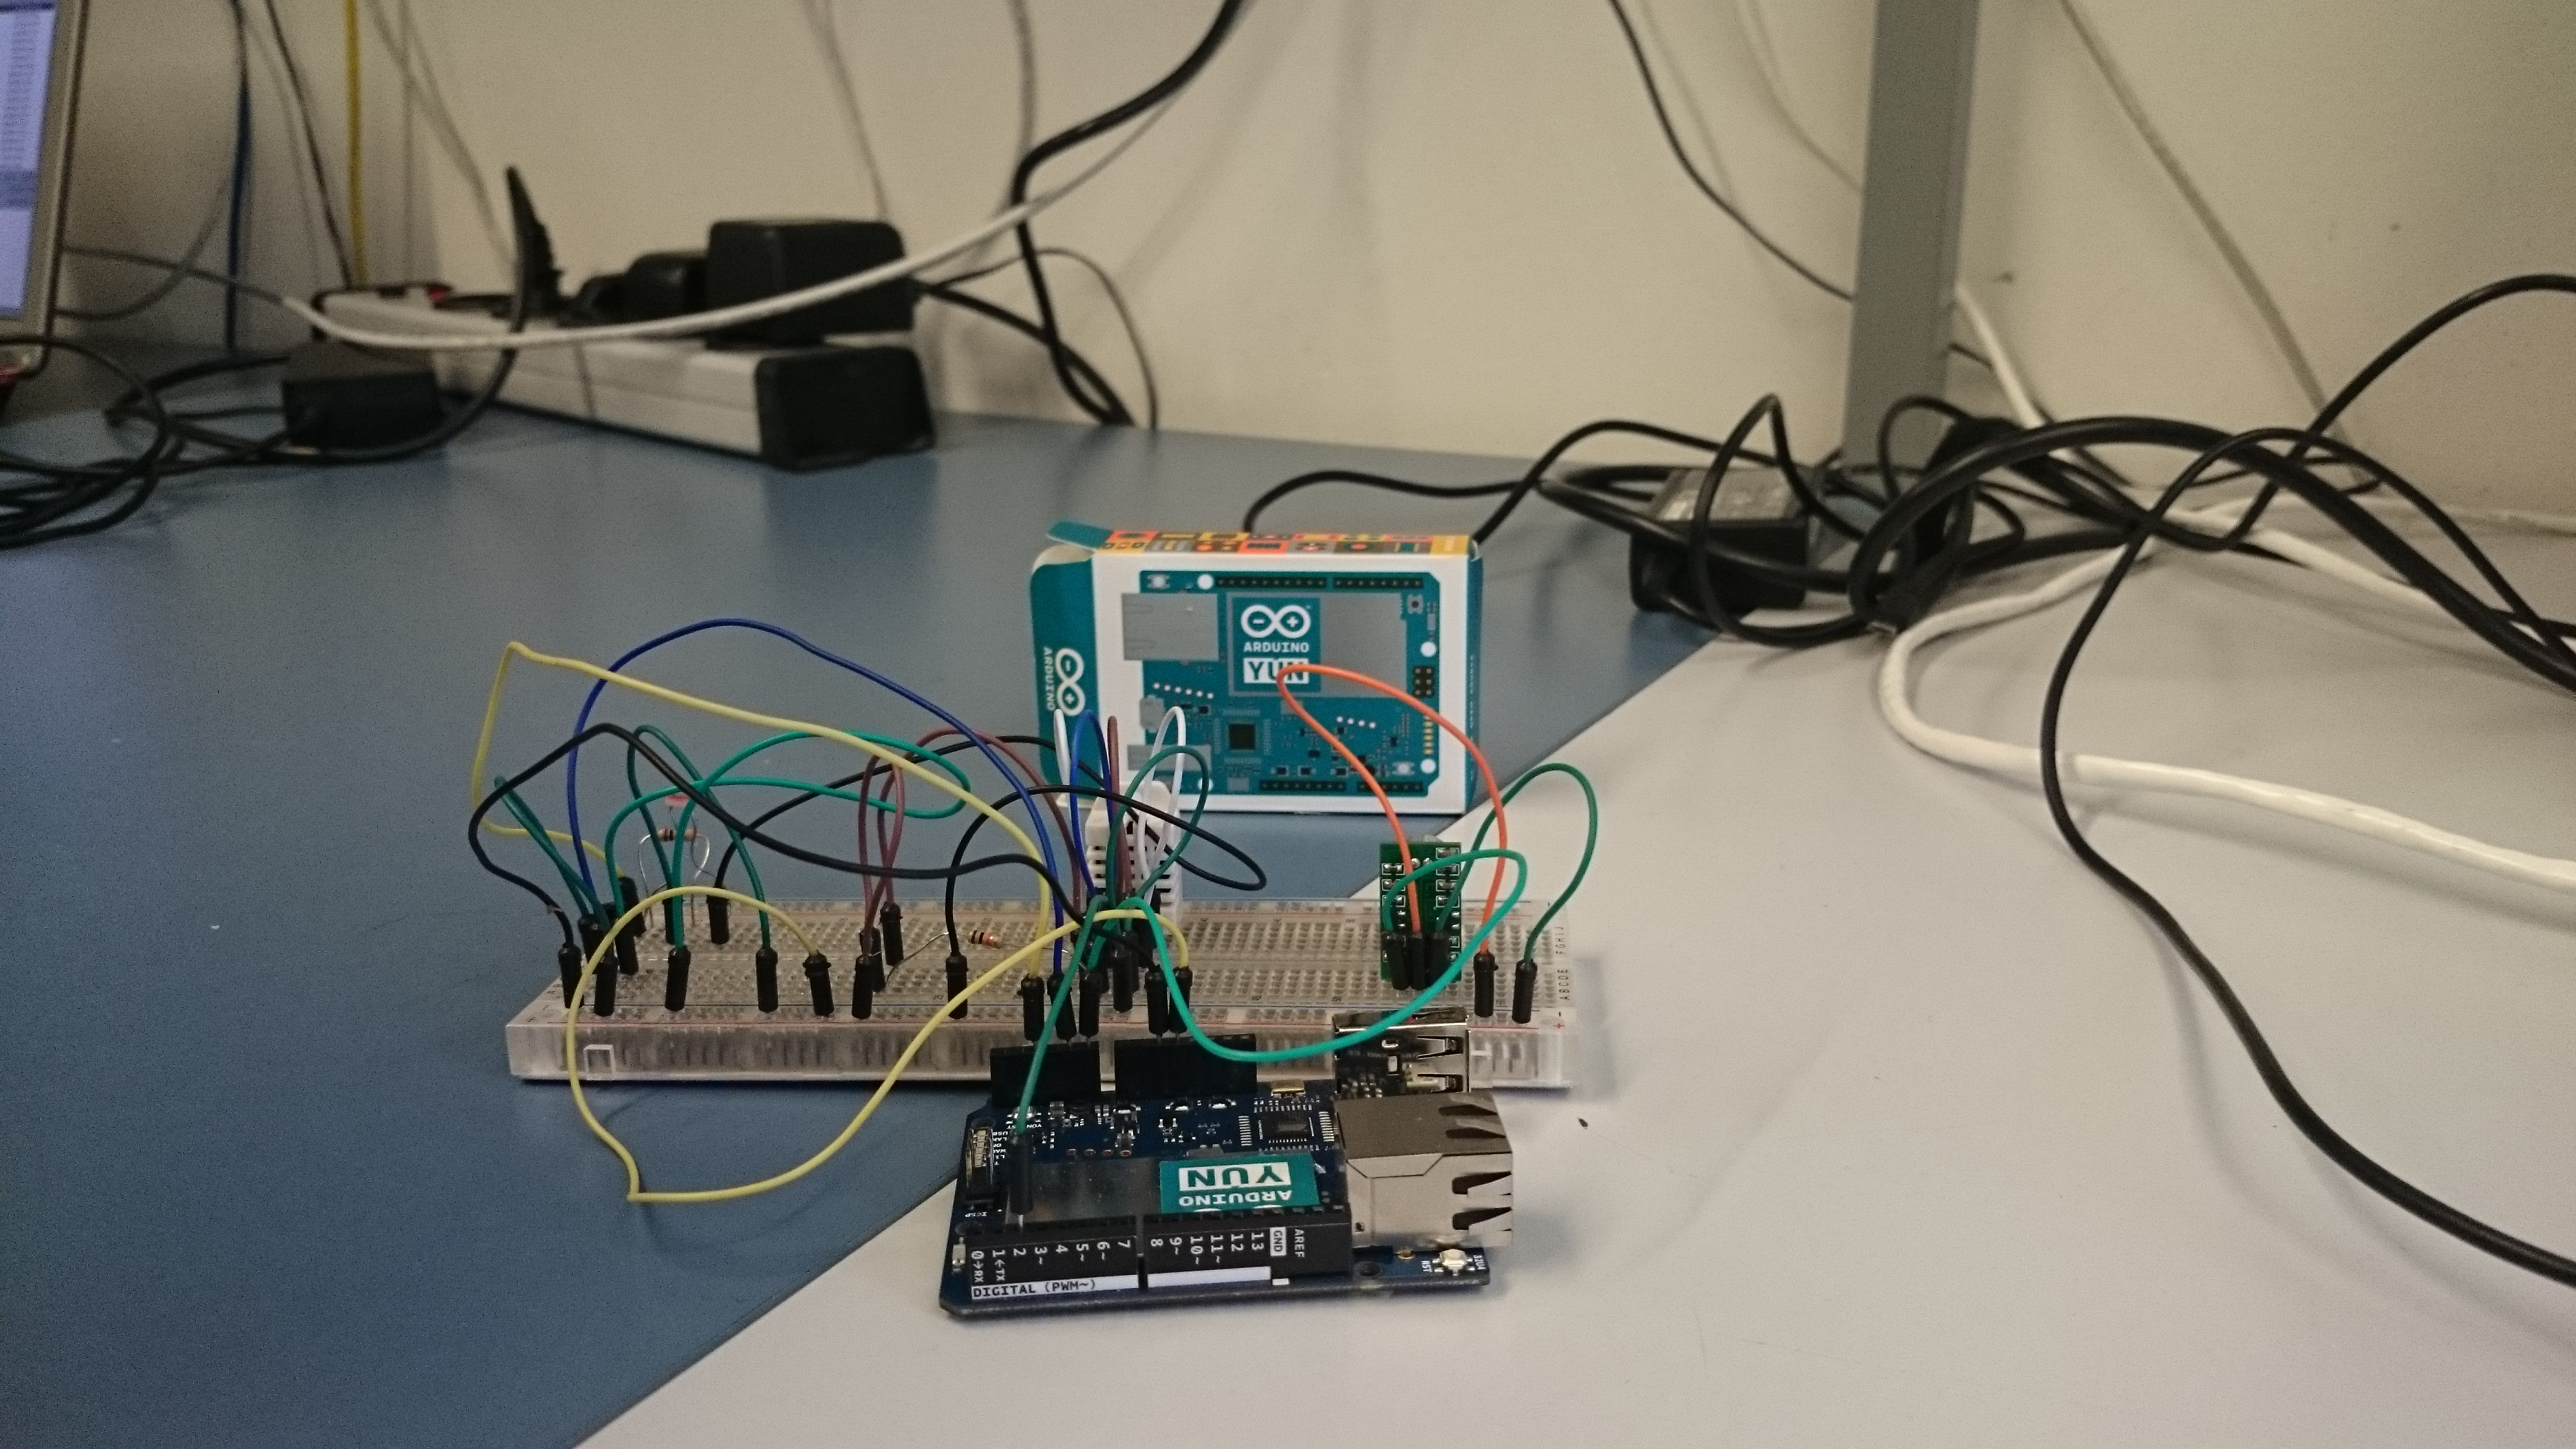
\includegraphics[scale=0.1]{./Figures/TestBed_Prototype.JPG}
          \rule{35em}{0.5pt}
      \caption[TestBed Prototype]{TestBed Prototype.}
      \label{fig:TestBed_Prototype}
  \end{figure} 
  
  \section{Sensor node}
  
  Now, I will show the process to configure the node, part of this process is taken of the website of Arduino\footnote{\url{http://arduino.cc/en/Guide/ArduinoYun}}:
  
  \subsection{Connection to the Internet}
    First of all an Internet connection has to be provide to the Arduino.
    \subsubsection{Through Ethernet}
      This is the fastest way to provide of Internet connection, the Arduino behave the same way as a computer, automatically receive an IP address.
      
    \subsubsection{Through WiFi}
      This is a slowest way. The process is the following:
      \begin{enumerate}
        \item First power the Arduino YUN. 
        \item The Arduino creates his own WiFi network (ArduinoYun-XXXXXXXXXXXX), and with a computer connect to it.
        \item When it is connected to the YUN network, go to a web browser and go to \url{http://arduino.local} or \url{192.168.240.1}. Put the password, which is ``arduino''. as shown in the figure \ref{fig:YunWebPassword}.
          \begin{figure}[htbp]
            \centering
                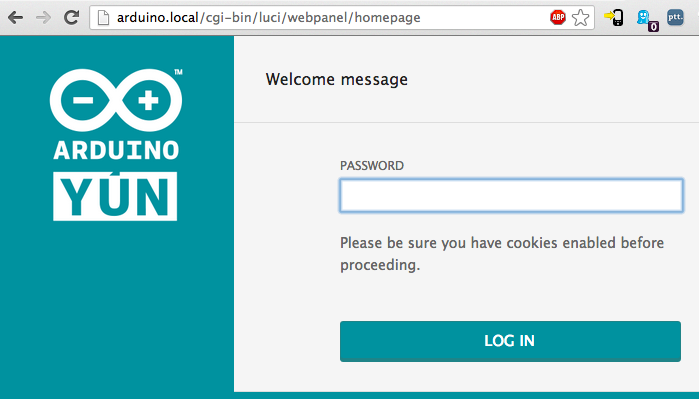
\includegraphics[scale=0.3]{./Figures/YunWebPassword.png}
                \rule{18em}{0.5pt}
            \caption[Yun web Password]{Yun web Password.}
            \label{fig:YunWebPassword}
          \end{figure}
        
        \item The next page is an information page, click on the configure button \ref{fig:YunWebDiagnostic}.
          \begin{figure}[htbp]
            \centering
                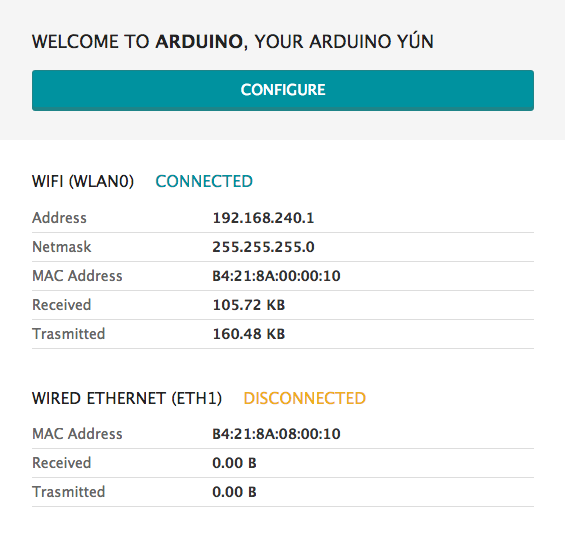
\includegraphics[scale=0.3]{./Figures/YunWebDiagnostic.png}
                \\
                \rule{15em}{0.5pt}
            \caption[Yun web Diagnostic]{Yun web Diagnostic.}
            \label{fig:YunWebDiagnostic}
          \end{figure}
        
        \item Give a unique name to the Yun, and the network to connect \ref{fig:YunWebConfig}.
          \begin{figure}[htbp]
            \centering
                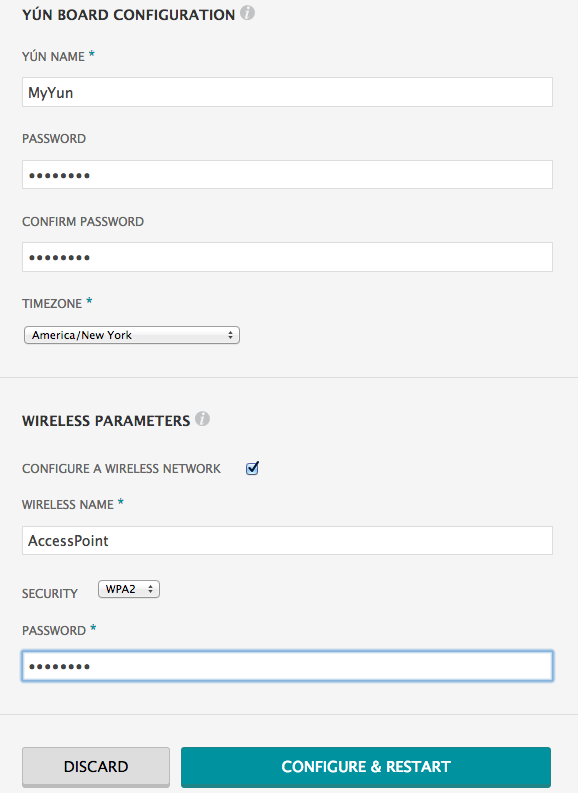
\includegraphics[scale=0.3]{./Figures/YunWebConfig.png}
                \\
                \rule{15em}{0.5pt}
            \caption[Yun web Configuration]{Yun web Configuration.}
            \label{fig:YunWebConfig}
          \end{figure}
          
        \item Press the configure \& restart button.
        \item Finally connect to the same network as the Yun is connected.
        
      \end{enumerate}
  \subsection{Install necessary packets}
    The Arduino will run an Arduino script and a python script, for python some packets have to be installed.
    
    To install any packet, connect to the Arduino (The password has to be ``arduino''):
    
    {\begin{centering} \textbf{ssh root@X.Y.Z.W}\par \end{centering}}
    
    Now install all the necessary packets:
     
      {\begin{centering} \textbf{
          opkg update \\
          opkg install distribute \\
          opkg install python-openssl \\
          easy\_install install geojson \\
          easy\_install install geopy \\
          easy\_install install httplib2
        }
      \par \end{centering}}
    
  \subsection{Copy the scripts}
    First of all it is necessary to create some directories, so once the ssh command has been done, go to ``/mnt/sda1'', make the following comands:
    
    {\begin{centering} \textbf{
    mkdir arduino \\
    cd arduino \\
    mkdir www \\
    }\par \end{centering}}
    
    Copy the python script ``main.py'' into the SD-Card. There are two ways to do this, putting the SDCard into a computer an saving the files in there, or copying the files into the Arduino through the network with the following comand:
    
    {\begin{centering} \textbf{
    scp main.py root@192.168.2.149:/mnt/sda1/arduino/www/main.py
    }\par \end{centering}}
  
  \subsection{Attach the sensors}
    Now that the python step is done, the sensors had to be attach the sensors to the Arduino Yun (Figure \ref{fig:AllSensors22_bb} or Figure \ref{fig:AllSensors11_bb}).
  
  \subsection{Arduino Code}
    To upload an Arduino sketch to the yun the IDE: Arduino 1.5.5 has to be used. There are two ways to upload an sketch, through an USB cable connected to the Arduino, or through the Internet. If we are in the same network as the Arduino, it will appear in the IDE.
  
  \section{Actual Testbed}
    We have three Arduinos, so we have to mount the sensor nodes and put them in three different places. The location should be in free space.
    
    When we have decided where we are going to put them, we have to introduce manually the location into the python script and the unique ID into the Arduino sketch. We can do that by entering into the Arduino by secure shell as it was explained earlier, go to the folder where the ``main.py'' is, and modified the following line by using ``nano'', a text editor:
    
    {\begin{centering} \textbf{self.address = 'Sagrada Familia, Carrer de Mallorca, Barcelona'}\par \end{centering}}
    
    After a day of collecting data, we got the Arduino's back, took the three logData files, and showed the data into some graphics.
    
    The figure \ref{fig:Testbedmap} shows the nodes deployed, the location try to be a little bit different to get distinc values.
    \begin{figure}[htbp]
      \centering
          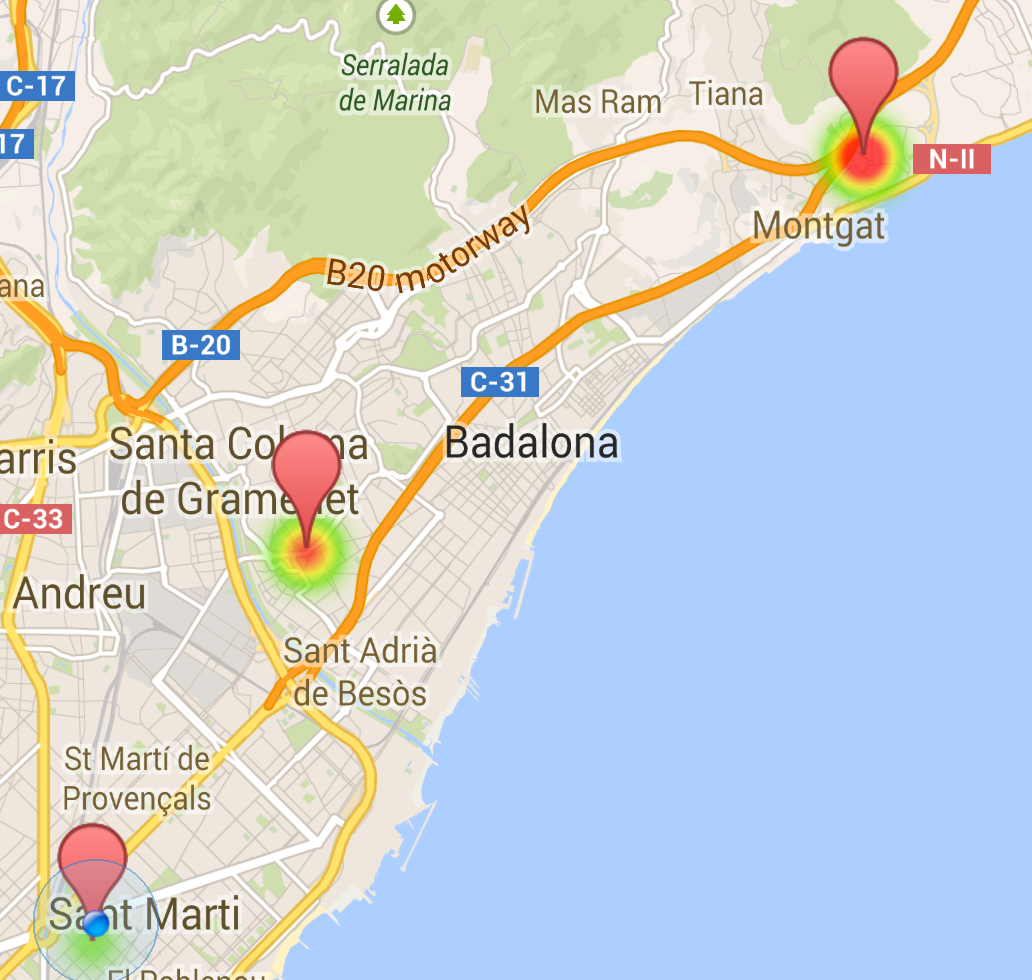
\includegraphics[scale=0.2]{./Figures/Testbedmap.png}
          \\
          \rule{15em}{0.5pt}
      \caption[Testbed Map]{Testbed Map.}
      \label{fig:Testbedmap}
    \end{figure}
    
    \subsection{Results}
      
      Thanks to the testbed a sensor network has been deployed, with only three nodes, for economical reasons, but it has been shown that the network could grow without problems.    
      
      A mobile application has been made, and shows an example that could led to more people to create other applications that work with the sensor data stored in Opencities. 
      The data has been stored on a platform and the mobile application has been able to access them, in this case a problem happened, the application was not designed to that amount of data, so it needs improvement.

      All the data produced during this testbed has been stored in the SD card of the Arduinos, and put them into graphics, as shown in the following figures: \ref{fig:GraphicTemperature}, \ref{fig:GraphicLight}, \ref{fig:GraphicNoise}, \ref{fig:GraphicHumidity}, \ref{fig:GraphicGas}.
      
      This graphics had been done with an octave script that analyze the logData file in every sensor node, but this graphics are only a portion of the real testbed, which has been place on Appendixes.
      
      \begin{figure}
        \centering
        \begin{subfigure}[b]{0.49\textwidth}
                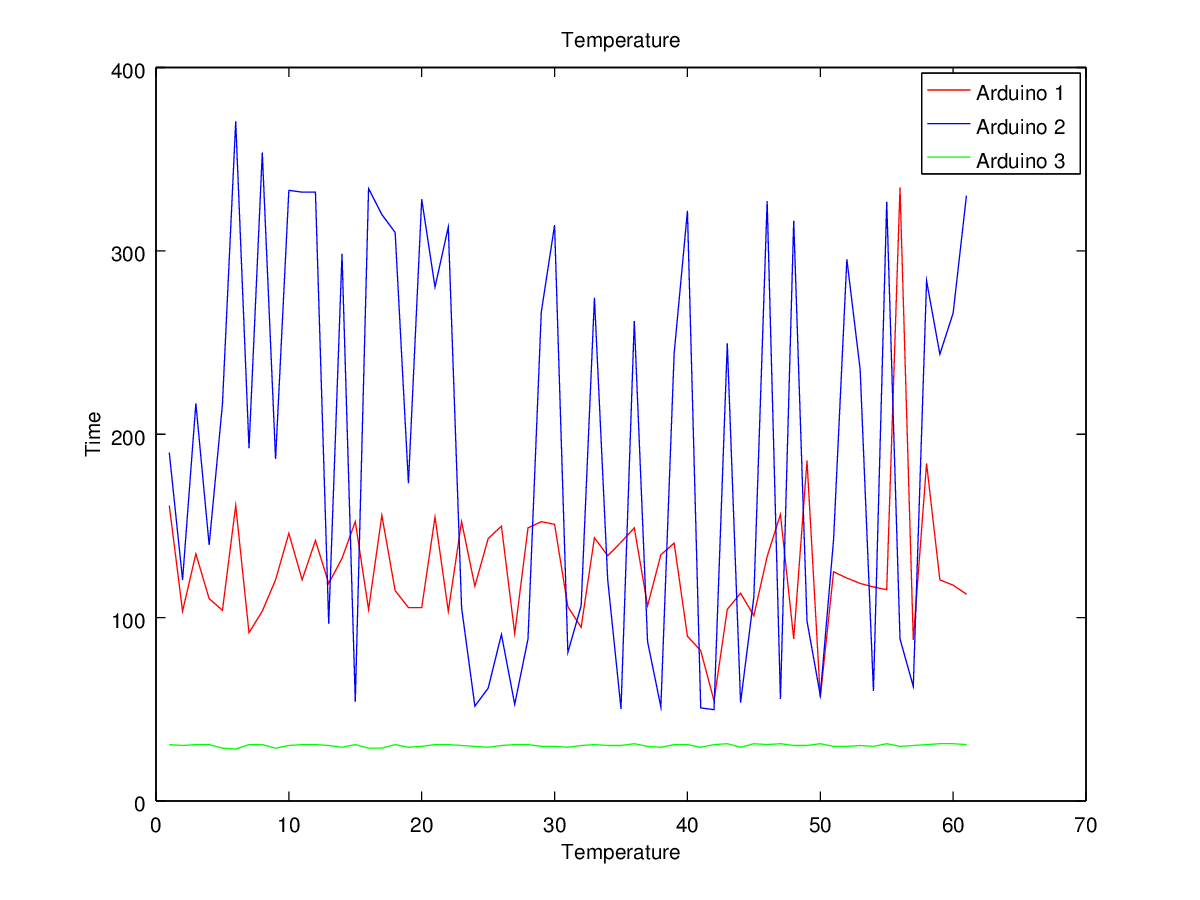
\includegraphics[width=\textwidth]{./Figures/GraphicTemperature.png}
                \caption{Graphic Temperature}
                \label{fig:GraphicTemperature}
        \end{subfigure}%
        ~ %add desired spacing between images, e. g. ~, \quad, \qquad, \hfill etc.
          %(or a blank line to force the subfigure onto a new line)
        \begin{subfigure}[b]{0.49\textwidth}
                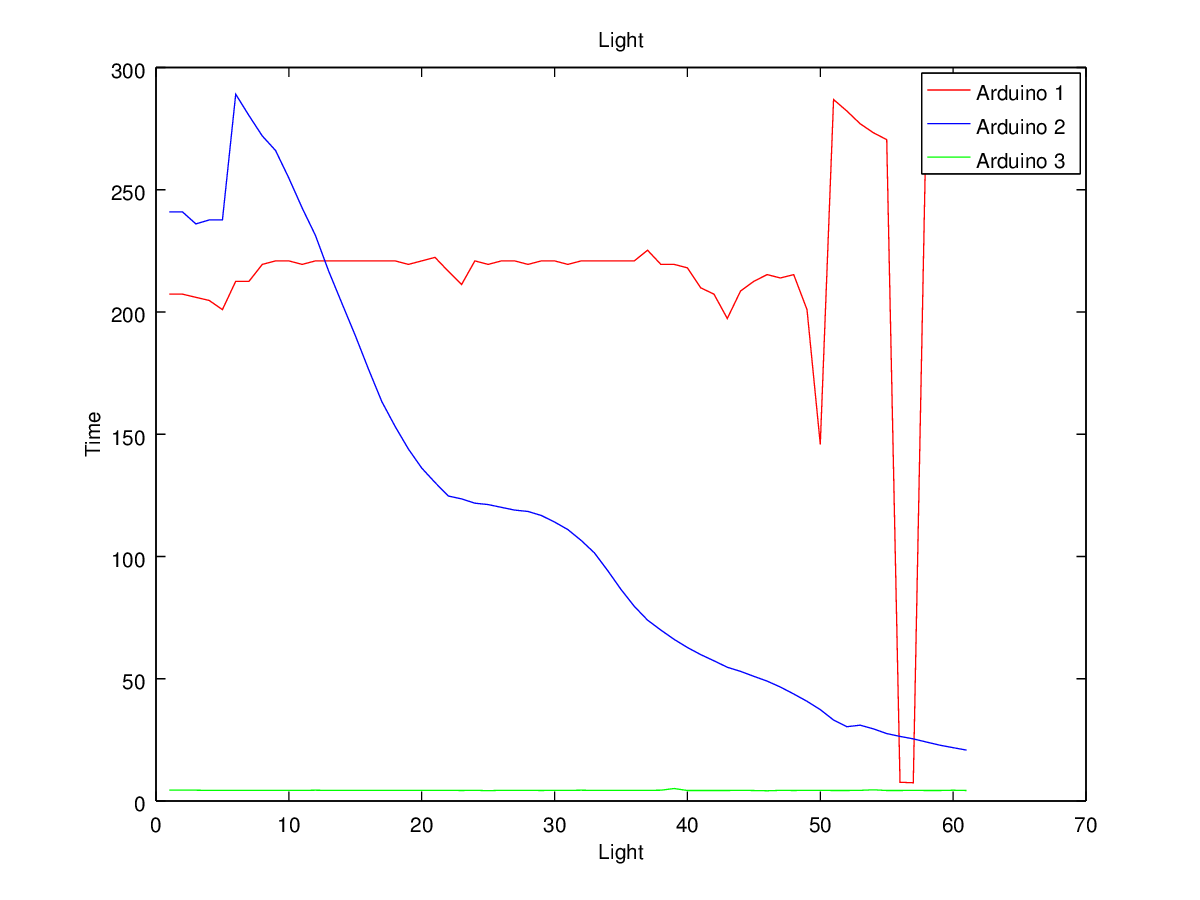
\includegraphics[width=\textwidth]{./Figures/GraphicLight.png}
                \caption{Graphic Light}
                \label{fig:GraphicLight}
        \end{subfigure}
        \rule{18em}{0.5pt}
        \caption{Testbed Results}\label{fig:TestbedResults1}
			\end{figure}
      
      \begin{figure}
        \centering
        \begin{subfigure}[b]{0.49\textwidth}
                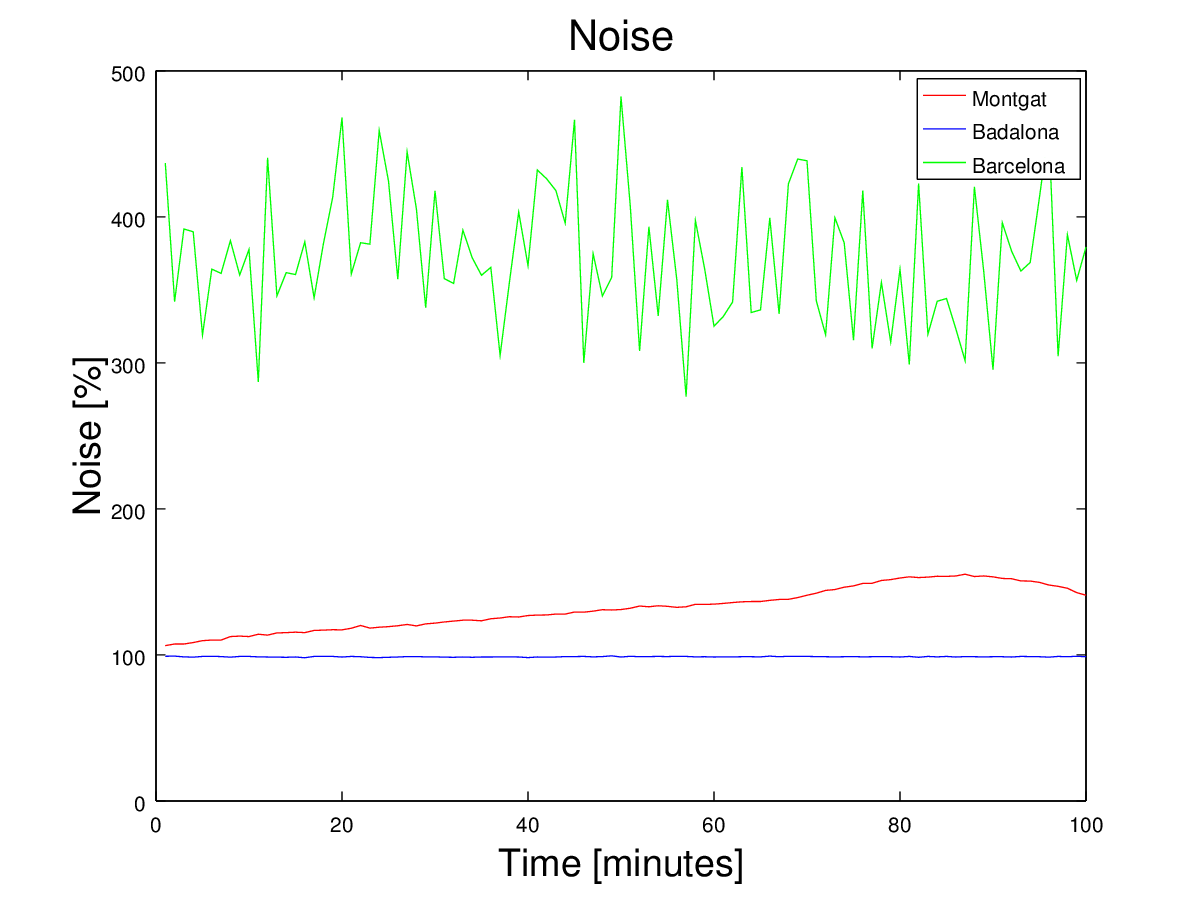
\includegraphics[width=\textwidth]{./Figures/GraphicNoise.png}
                \caption{Graphic Noise}
                \label{fig:GraphicNoise}
        \end{subfigure}%
        ~ %add desired spacing between images, e. g. ~, \quad, \qquad, \hfill etc.
          %(or a blank line to force the subfigure onto a new line)
        \begin{subfigure}[b]{0.49\textwidth}
                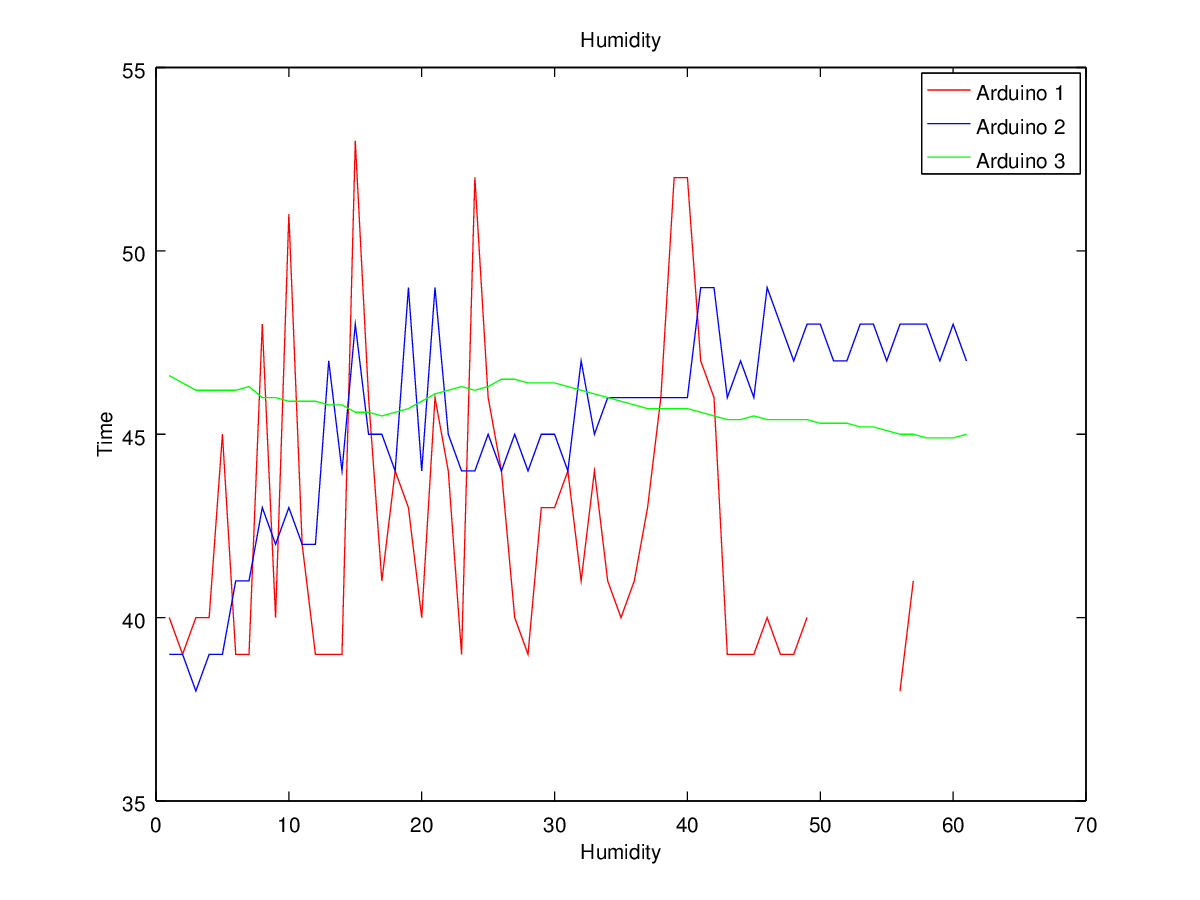
\includegraphics[width=\textwidth]{./Figures/GraphicHumidity.png}
                \caption{Graphic Humidity}
                \label{fig:GraphicHumidity}
        \end{subfigure}
        \rule{18em}{0.5pt}
        \caption{Testbed Results}\label{fig:TestbedResults1}
			\end{figure}
      
      \begin{figure}[htbp]
		    \centering
		        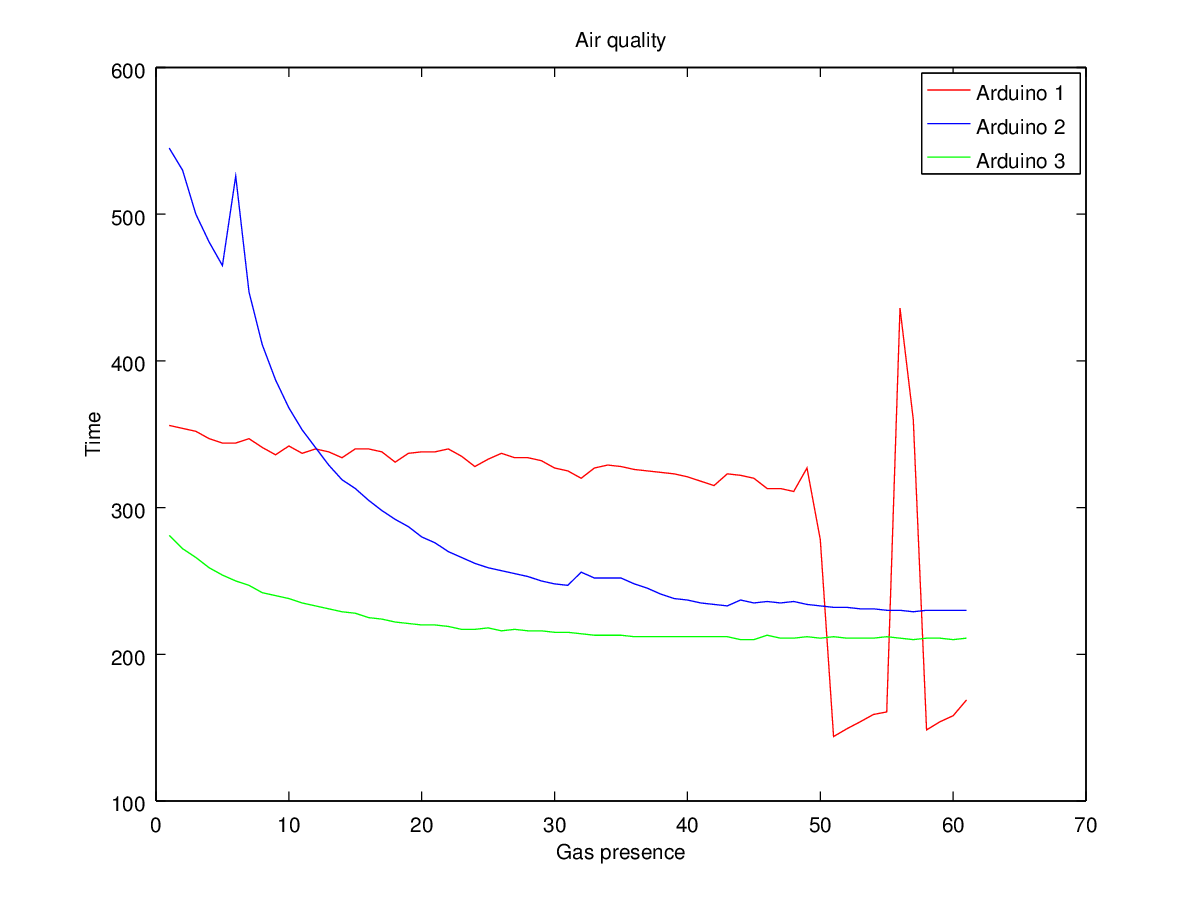
\includegraphics[scale=0.5]{./Figures/GraphicGas.png}
		        \caption[Graphic Air Quality]{Graphic Air Quality.}
		        \label{fig:GraphicGas}
		    \label{fig:Testbedmap}
		  \end{figure}
		  
		  Graphics explanation:
    
\chapter{Conclusions}
\label{Chapter6}
  
  During this project a deployment of a sensor network had been made with optimal results, this has proved that the sensor nodes have properly.
  
  Therefore, it has been shown that anyone can deploy its own network in an inexpensive way, with open source, and easy to use.
  
  A mobile application has been developed to serve as an example, so the citizens who want to create their own find the process easier.
  
  All the code that it has been created during this project is open source and is online, in a Github repository.

  In conclusion, the project had satisfied the goals presented at the start, which are share sensor data on an open network, and let the users visualize it.

\chapter{Future work}
\label{Chapter7}
  
  This project can be improved in two ways, the sensor node and the Android application.
  
  In the case of the sensor node it will be best if a prototype is build for the node to be in the outside, and, also to make the Arduino Power over Ethernet.
  
  On the other hand, the mobile application showed some issues, when the data is too big, the process takes a little bit, which could make the users stop using it. But there is also a line that could not be make in this project, and is to show how the data changes during a period of time.
  
  Finally, there has not been any difusion of the project, in the future, the project could be difuse by a webpage or conference on sensors.

\bibliography{bibliography}
\phantomsection
\addcontentsline{toc}{chapter}{BIBLIOGRAPHY}
\cleardoublepage

\chapter{Appendixes}
\label{Chapter8}

  \section{Pilot Charter}
\label{sec:mnp}

Fellow: Sergio Almendros Diaz
\\
Mentor: 
\\
Advisor: Jaume Barcelo

\subsection{Pilot purpose or justification}
The purpose of this pilot is to build a sensor platform that can be attached to guifi nodes to gather and share sensory data.

\subsection{Measurable pilot objectives and related success criteria}
\begin{itemize}
\item Gather data about temperature, humidity, light, and noise. 
\item Share the data as open data.
\item Deploy at least two nodes and gather data for at least two weeks.
\end{itemize}

\subsection{High-level requirements}
\begin{itemize}
\item Outdoor enclosure.
\item Use open hardware and open software to the possible extent.
\item Use standardized interfaces to integrate with other projects.
\end{itemize}

\subsection{High-level pilot description}
The goal is to use an arduino platform to create a bottom-up broadband wireless sensor networks. 
As guifi.net has already over 20,000 nodes, the idea is to co-locate the sensory platforms together with the guifi.net nodes and use the guifi.net network to transmit the data.
This data should be gathered and shared.
Ideally, the pilot should include a presentation interface for the users to visualize the data.

\subsection{High-level risks}
A possible risk is that the prototypes are not rugged enough for outdoor environments.
It is also a risk that the prototype is not stable and needs to be reset very often.

\subsection{Summary milestone schedule}
\begin{itemize}
\item From 20/09/2013 to 23/09/2013
	\begin{itemize}
	\item Establish the general idea of the TFG and specifics goals.
	\end{itemize}
\item From 23/09/2013 to 11/10/2013
	\begin{itemize}
	\item Specify the tasks to do and make a planning.
	\end{itemize}
\item From 11/10/2013 to 30/10/2013
	\begin{itemize}
	\item Connect first sensors to the Arduino.
	\end{itemize}
\item From 31/10/2013 to 10/01/2014
	\begin{itemize}
	\item Connect to guifi network and upload data to an open data platform.
	\end{itemize}
\item From 10/01/2014 to 01/06/2014
	\begin{itemize}
	\item Integration of sensors and communication aspects.
	\item Install prototypes.
	\item Data sharing and visualization.
    \item Data analysis and evaluation of the testbed.
	\end{itemize}
\item From 02/06/2014 to 30/06/20014
	\begin{itemize}
	\item Preparation of the final memory.
	\end{itemize}
\item From 01/07/2014 to the date of the presentation
	\begin{itemize}
	\item Make the presentation.
	\end{itemize}
\end{itemize}

\subsection{Summary budget}
The cost of this pilot will be approximately 4000 \euro. This quantity is for the scholarship to the student that will develop this pilot, budget for attending a conference or visiting collaborators, and the purchase of the necessary hardware.

  \documentclass[10pt,a4paper]{article}
\usepackage{pgfgantt}

\title{A bottom up sensor testbed}
\author{Sergio Almendros Diaz}
\date{\today}

\begin{document}
\maketitle

\section{Planning Report}

The following sections explain the tasks that I will do in the course of this project.

\subsection{Familiarization with the Arduino Yun}

In this project I will be working with an arduino Yun, but I never worked before with any type of arduino, so the first task is to start coding different kind of programs. Then I will have to learn how to interact with the linux in the arduino Yun.

\subsection{Small problem solution}

I want to do an easy example to how to connect an arduino with a server running in my computer, what I want to do is establish a bridge between an arduino program and the linux within the arduino to be able to communicate with a server in my laptop, and send a string with the value returned by a sensor.
This is a reduce problem of the real "bottom-up sensor testbed" because, at the end, in every arduino will be a program that will have to send a message to a server with the data of the sensors attached to it.

\subsection{Collect Data from sensors}

First I will connect a temperature sensor to the arduino YUN, then, I will develop a program to collect the information from it, and send it to a server.
When the temperature sensor works, I will do the same process with a humidity, light, and noise sensor.

\subsection{Install Sentilo}

Sentilo (www.sentilo.io) is an open source sensor and actuator platform that I will install in my laptop to act as the server between the sensor network and the interface for the users to visualize the data. 

\subsection{Communication with Sentilo}

I will adapt the messages that the arduino send to fit with the Sentilo.

\subsection{Real deployment}

At this moment, the part of the arduino and the server will be done, so I will test the server installing the arduino in real nodes of the guifi network, for example, the node in the Universitat Pompeu Fabra, and any other node that allow me to install it. The arduino will have a temperature, humidity, light, and noise sensor.

\subsection{Interface}

I want to do an interface for any user to understand the meaning of the temperature, humidity, light, and noise values. This interface will be develop for an android mobile application.

\subsection{Sentilo module}

I will contribute to Sentilo and other sensor data brokerage platforms accommodating the sensor testbed deployed in the previous tasks.

\subsection{Final report}

This task have to be done in parallel with all the other ones, and its purpose is document all the work that I will do.

\subsection{Gantt chart}

\begin{figure}
\begin{center}
  \begin{ganttchart}{1}{23}
    \gantttitle{Pilot Timeline}{23} \\ 
    \ganttbar{Task 1 [7/01/14 - 12/01/14]}{1}{1} \\
    \ganttlinkedbar{Task 2 [13/01/14 - 19/01/14]}{3}{4} \\
    \ganttlinkedbar{Task 3 [20/01/14 - 2/02/14]}{5}{7} \\
    \ganttlinkedbar{Task 4 [3/02/14 - 5/02/14]}{8}{8} \\
    \ganttlinkedbar{Task 5 [6/02/14 - 16/02/14]}{9}{11} \\
    \ganttlinkedbar{Task 6 [17/02/14 - 2/03/14]}{12}{13} \\
    \ganttlinkedbar{Task 7 [3/03/14 - 30/04/14]}{14}{18} \\
    \ganttlinkedbar{Task 8 [1/05/14 - 31/06/14]}{19}{22} \\
    \ganttbar{Task 9 [7/01/14 - 31/06/14]}{1}{22}
  \end{ganttchart}
\end{center}
\end{figure} 
 

\end{document}

  \section{Class Diagram}
  
  	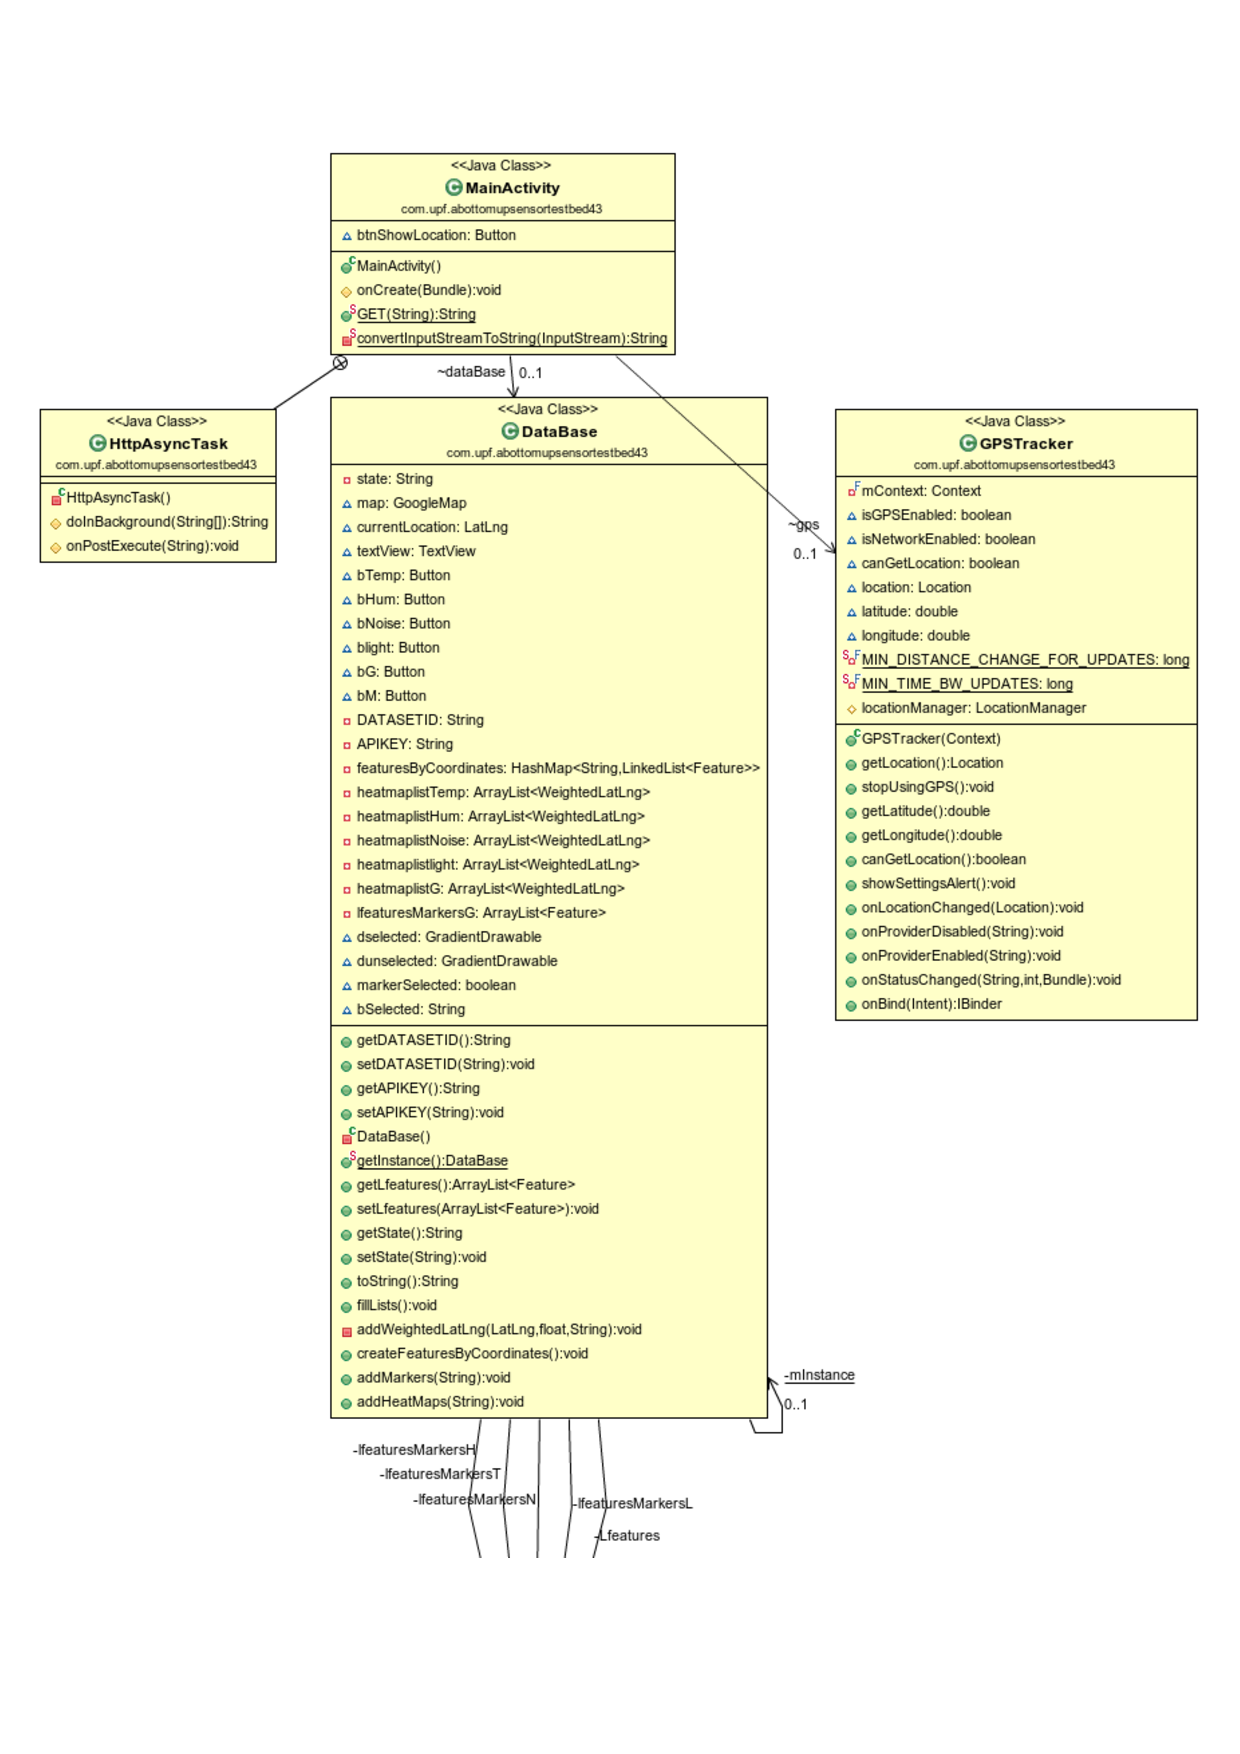
\includepdf[]{./AdditionalInformation/ClassDiagram1_1.pdf}

    \begin{figure}[H]
      \centering
        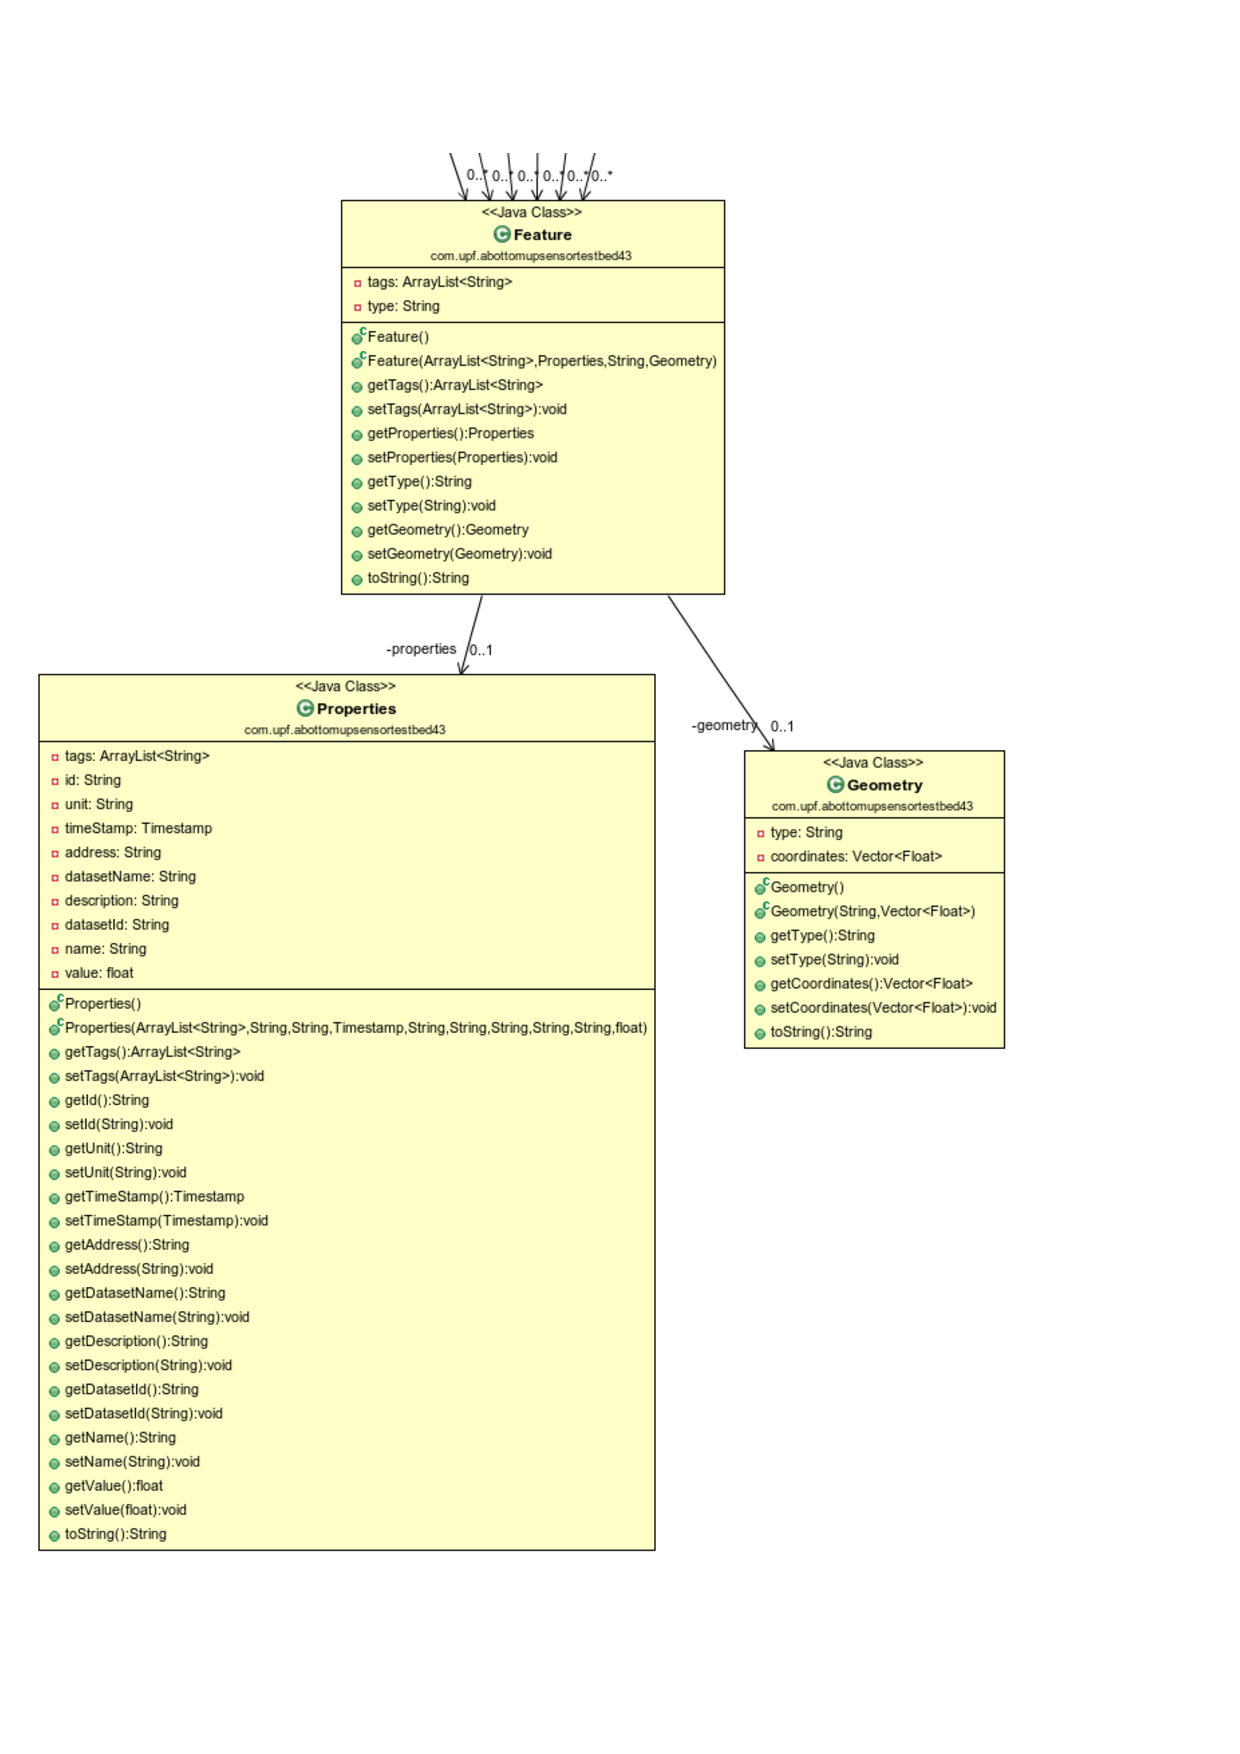
\includegraphics[page=1,scale=0.8]{./AdditionalInformation/ClassDiagram1_2.pdf}
      \rule{35em}{0.5pt}
      \caption[Class Diagram of the Android App part 2]{Class Diagram of the Android App part 2.}
      \label{fig:ClassDiagram2}
    \end{figure}
  
  \section{Testbed Graphics}
  	\begin{figure}[H]
      \centering
        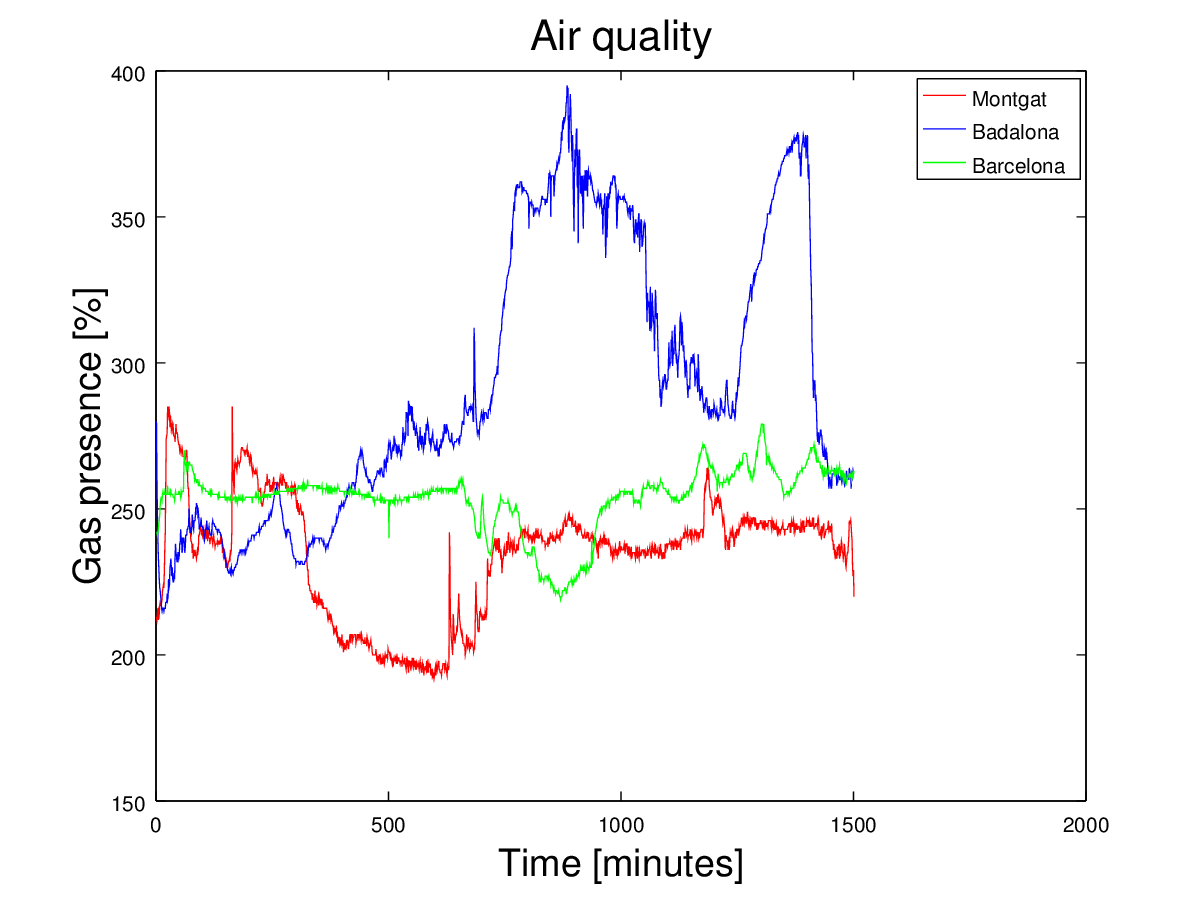
\includegraphics[page=1,scale=0.8]{./Figures/CompleteGraphicGas.png}
      \rule{35em}{0.5pt}
      \caption[Complete Graphic Air Quality]{Complete Graphic Air Quality.}
      \label{fig:CompleteGraphicGas}
    \end{figure}
    
    \begin{figure}[H]
      \centering
        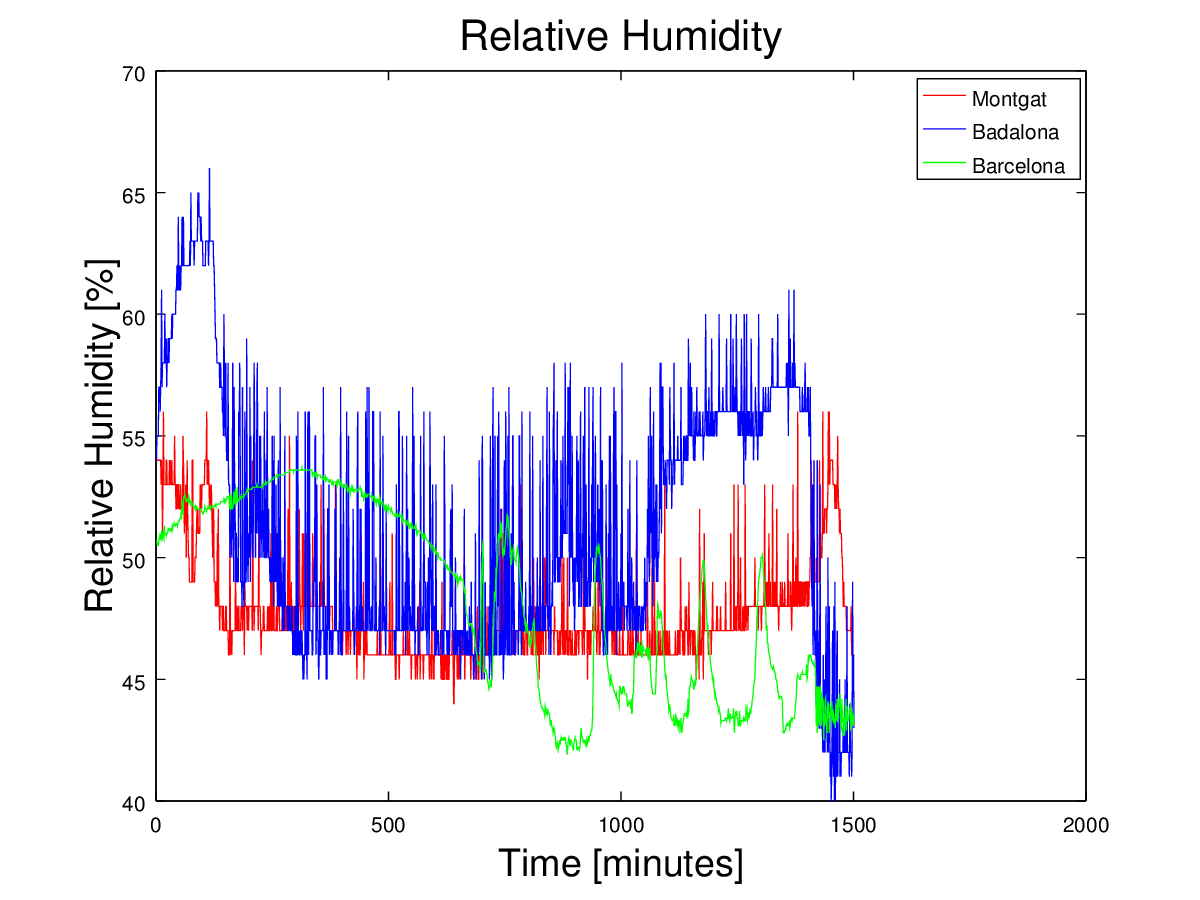
\includegraphics[page=1,scale=0.8]{./Figures/CompleteGraphicHumidity.png}
      \rule{35em}{0.5pt}
      \caption[Complete Graphic Humidity]{Complete Graphic Humidity.}
      \label{fig:CompleteGraphicHumidity}
    \end{figure}
    
    \begin{figure}[H]
      \centering
        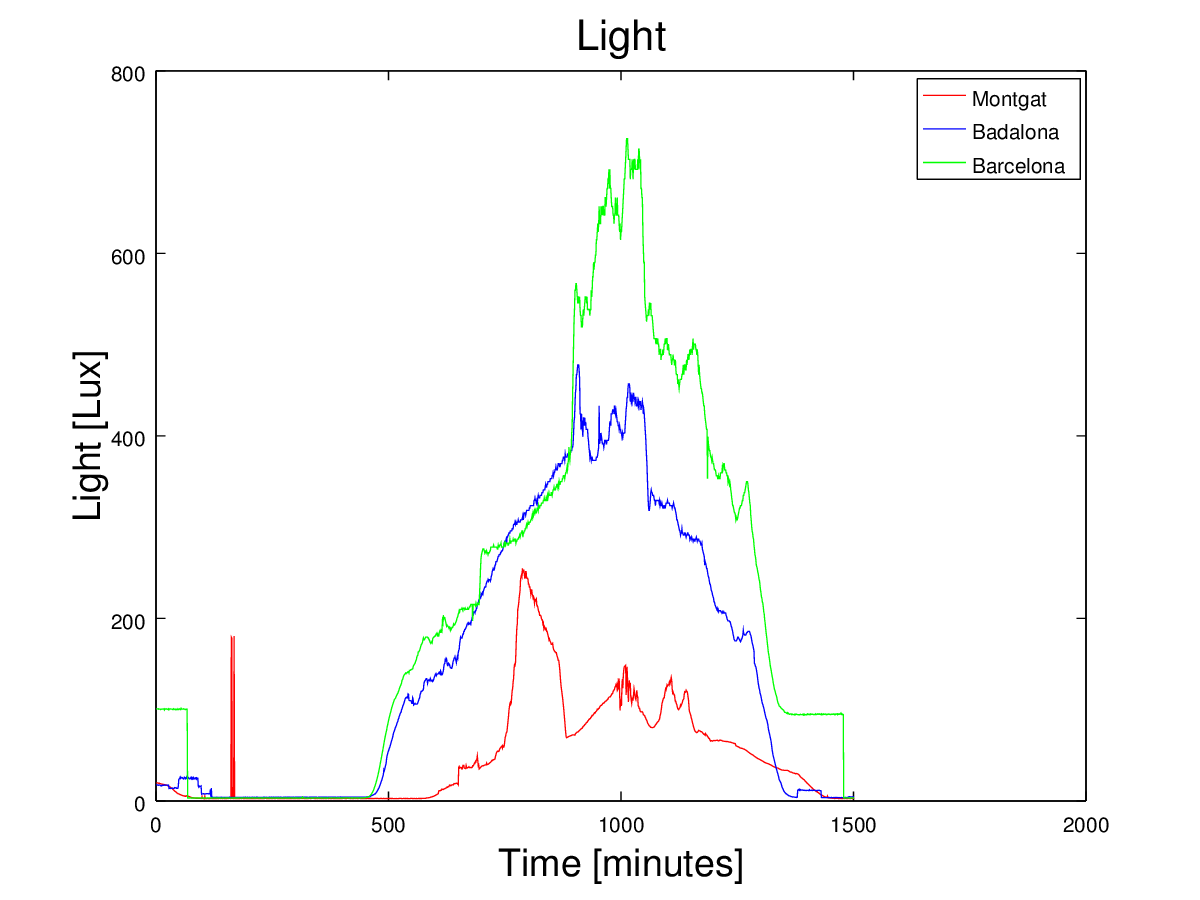
\includegraphics[page=1,scale=0.8]{./Figures/CompleteGraphicLight.png}
      \rule{35em}{0.5pt}
      \caption[Complete Graphic Light]{Complete Graphic Light.}
      \label{fig:CompleteGraphicLight}
    \end{figure}
    
    \begin{figure}[H]
      \centering
        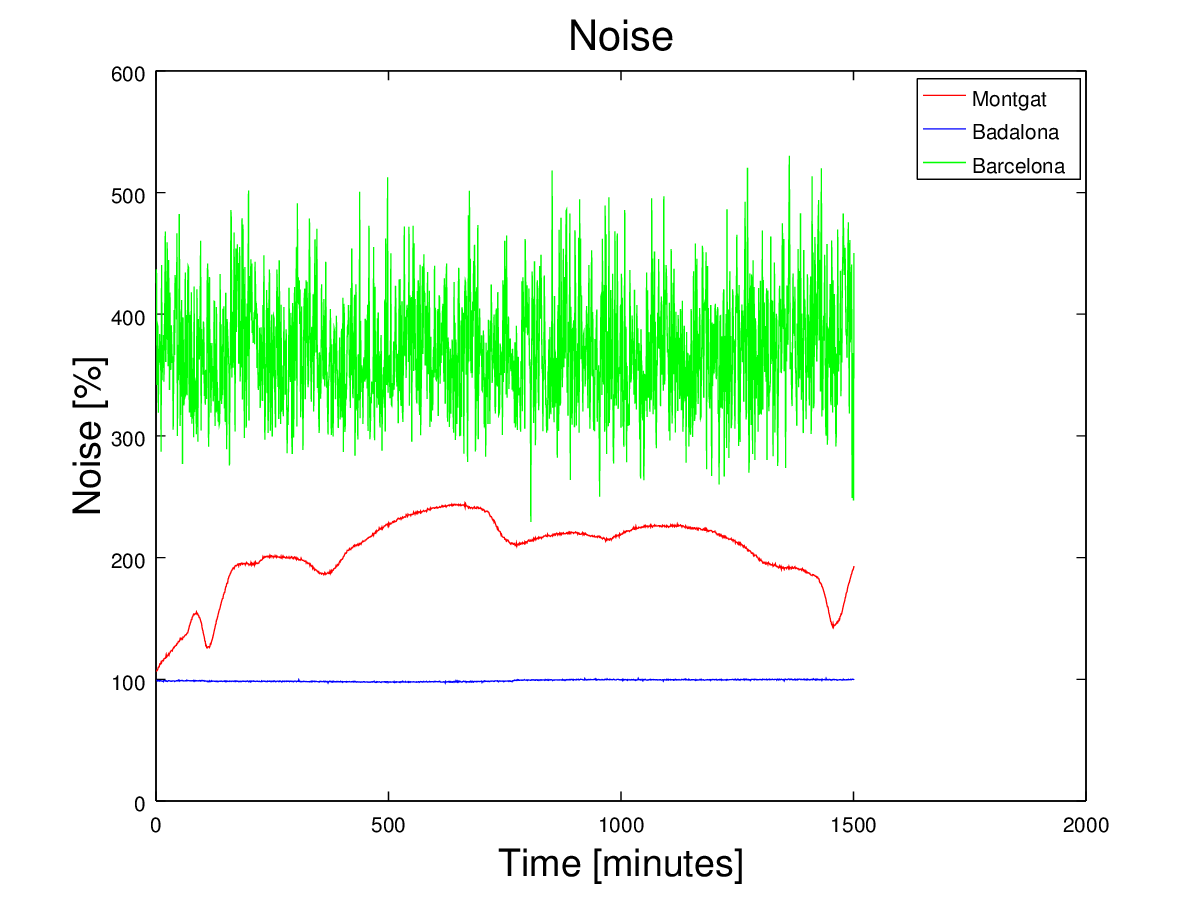
\includegraphics[page=1,scale=0.8]{./Figures/CompleteGraphicNoise.png}
      \rule{35em}{0.5pt}
      \caption[Complete Graphic Noise]{Complete Graphic Noise.}
      \label{fig:CompleteGraphicNoise}
    \end{figure}
    
    \begin{figure}[H]
      \centering
        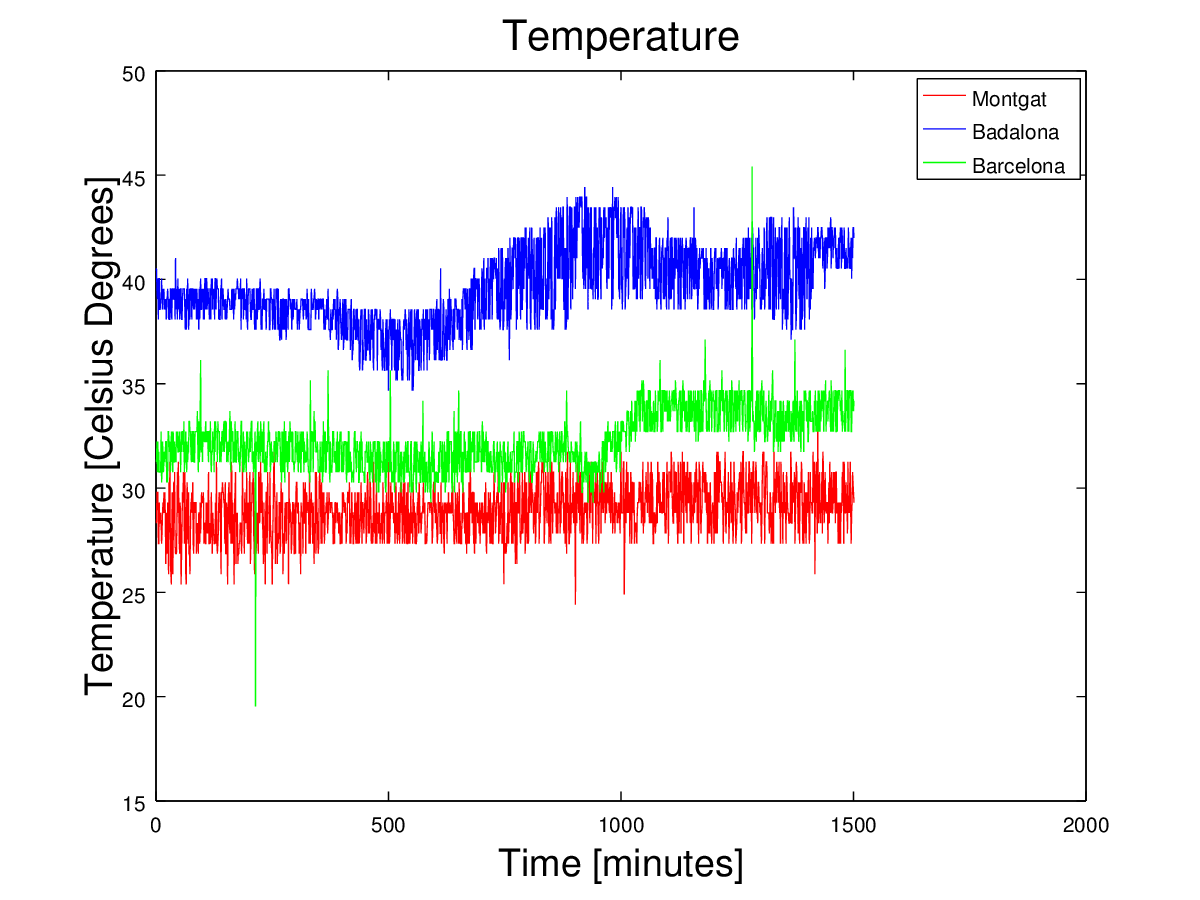
\includegraphics[page=1,scale=0.8]{./Figures/CompleteGraphicTemperature.png}
      \rule{35em}{0.5pt}
      \caption[Complete Graphic Temperature]{Complete Graphic Temperature.}
      \label{fig:CompleteGraphicTemperature}
    \end{figure}
  


\backmatter
\printindex





\end{document}


%NUMERACI� DE LA P�GINA EXTERIOR EXCEPTE EN LA PRIMERA P�GINA DE CADA CAP�TOL
\usepackage{fancyhdr}
\pagestyle{fancy}
\fancyfoot{}
\fancyfoot[RO]{\thepage}
\fancyfoot[LE]{\thepage}


%MUTIPLES �NDEX
%En el pre�mbul
\usepackage{multind}
\makeindex{authors}
%Introducci� d'entrades la forma
\index{authors}{Einstein}
%Situaci� de l'�ndex
\printindex{authors}{Author index}
%Cal eliminar les comandes \usepakage{makeidx} \makeindex \printindex
%cal exacutar des de la l�nia de comandes makeindex authors
